\documentclass[a4paper,11pt,dvipdfmx,uplatex]{jsbook}
\usepackage{docmute}
%\usepackage{fancyhdr}
\setlength{\footskip}{16pt}
\usepackage{amsmath}
\usepackage[dvipdfmx]{graphicx}
\usepackage[dvipdfmx]{color}
%\usepackage{pagecolor}[white]
\usepackage{amsmath,amssymb}
%\usepackage[top=3cm, bottom=3cm, left=3cm, right=3cm]{geometry}
\usepackage{braket}
\usepackage{bm}
\numberwithin{equation}{section}
\usepackage{mathrsfs}
\usepackage{siunitx}
\usepackage{physics}
\usepackage[dvipdfmx]{graphicx}
\usepackage[compat=1.1.0]{tikz-feynhand}
\usepackage{caption}
\usepackage{subcaption}
%\usepackage{cleveref}
\usepackage{float}
\usepackage{multicol}
\setlength{\columnsep}{15mm}
%\usepackage[style=phys,articletitle=false,biblabel=brackets,chaptertitle=false,pageranges=false]{biblatex}
%\usepackage[style=phys]{biblatex}
\usepackage[dvipdfmx]{hyperref}
\usepackage{url}
\usepackage{pxjahyper}
\usepackage{bookmark}
%\usepackage[backref]{hyperref}
\setcounter{tocdepth}{3}
\setlength{\parindent}{2em}
\def\vector#1{\mbox{\boldmath $#1$}}
\def\slash#1{\not\!#1}
\def\slashb#1{\not\!\!#1}
\def\delsla{\not\!\partial}
%\usepackage[dvipdfmx]{xcolor}


\hypersetup{
 setpagesize=false,
 bookmarksnumbered=true,%
 bookmarksopen=true,%
 colorlinks=true,%
 linkcolor=black,
 citecolor=red,
 urlcolor=black,
}
%backreferenceのカスタマイズ. "Back to p.3"のように表示する.
%\renewcommand*{\backref}[1]{(p.#1へ戻る)}
%\newcommand{\backtoc}{\hyperlink{toc}{[目次へ]}}
\newcommand{\backtoc}{\texorpdfstring{\protect\hyperlink{toc}{\hspace{5pt} \scriptsize [目次へ]}}{}}
\newcommand{\mychapter}[1]{\chapter[#1]{#1\backtoc}}
\newcommand{\mysection}[1]{\section[#1]{#1\backtoc}}
\newcommand{\mysubsection}[1]{\subsection[#1]{#1\backtoc}}
\usepackage[style=phys,articletitle=false,biblabel=brackets,chaptertitle=false,pageranges=false,abbreviate=true]{biblatex}
\addbibresource{ref.bib}
\DefineBibliographyStrings{english}{
  andothers = {\emph{et al.}} % "and others" を斜体の "et al." に変更
}
\renewcommand{\bibname}{参考文献} % レポートや書籍の場合
\renewcommand{\refname}{参考文献} % 論文や記事の場合


\thispagestyle{empty} %ページ番号をつけない場合

              % ここから本文が始まる
\makeatletter

\def\@thesis{修士論文}
\def\id#1{\def\@id{#1}}
\def\master#1{\def\@master{#1}}
\def\department#1{\def\@department{#1}}

\def\@maketitle{
\begin{center}
{\Large \@thesis \par} %修士論文と記載される部分
\vspace{25mm}
{\Large \@title \par}% 論文のタイトル部分
\vspace{10mm}
{\LARGE\bf\@department\par} % 提出年月日部分j
\vspace{10mm}
{\Large 提出日\@date \par} % 所属部分
\vspace{80mm}
{\Large \@master \par} % 学年部分
\vspace{10mm}
{\Large 学籍番号 \@id \par} % 学籍番号部分
\vspace{10mm}
{\Large 氏名 \@author}% 氏名
\end{center}
%\par\vskip 1.5em
}

\everymath{\rm}

\begin{document}    
\makeatother
\title{\vspace{-80pt}修士論文\\[35pt]電子ビームエネルギー精密測定のための\\アンジュレータ放射光干渉法\\[30pt]{\Large Undulator radiation interferometry\\for electron beam energy measurement}}
\date{令和7年 (2025年)}
\department{東京大学大学院理学系研究科物理学専攻中村哲研究室}
\id{35-236076}
\master{修士2年}
%\vspace{700pt}
\author{\\[150pt]東京大学大学院 理学研究科 物理学専攻\\中村哲研究室\\\\西 幸太郎}

\maketitle
\setlength{\abovedisplayskip}{20pt} 
\setlength{\belowdisplayskip}{20pt}
\hypertarget{toc}{}
%\hypertarget{toc}{}
\tableofcontents
\listoffigures
\listoftables
%\section[章]{章\texorpdfstring{\protect\hyperlink{toc}{\hspace{5pt} \small [目次へ]}}{}}
%\section[章]{章\backtoc}
%\documentclass[a4paper,11pt,uplatex]{jsbook}

%\usepackage{fancyhdr}
\setlength{\footskip}{16pt}
\usepackage{amsmath}
\usepackage[dvipdfmx]{graphicx}
\usepackage[dvipdfmx]{color}
%\usepackage{pagecolor}[white]
\usepackage{amsmath,amssymb}
%\usepackage[top=3cm, bottom=3cm, left=3cm, right=3cm]{geometry}
\usepackage{braket}
\usepackage{bm}
\numberwithin{equation}{section}
\usepackage{mathrsfs}
\usepackage{siunitx}
\usepackage{physics}
\usepackage[dvipdfmx]{graphicx}
\usepackage[compat=1.1.0]{tikz-feynhand}
\usepackage{caption}
\usepackage{subcaption}
%\usepackage{cleveref}
\usepackage{float}
\usepackage{multicol}
\setlength{\columnsep}{15mm}
%\usepackage[style=phys,articletitle=false,biblabel=brackets,chaptertitle=false,pageranges=false]{biblatex}
%\usepackage[style=phys]{biblatex}
\usepackage[dvipdfmx]{hyperref}
\usepackage{url}
\usepackage{pxjahyper}
\usepackage{bookmark}
%\usepackage[backref]{hyperref}
\setcounter{tocdepth}{3}
\setlength{\parindent}{2em}
\def\vector#1{\mbox{\boldmath $#1$}}
\def\slash#1{\not\!#1}
\def\slashb#1{\not\!\!#1}
\def\delsla{\not\!\partial}
%\usepackage[dvipdfmx]{xcolor}


\hypersetup{
 setpagesize=false,
 bookmarksnumbered=true,%
 bookmarksopen=true,%
 colorlinks=true,%
 linkcolor=black,
 citecolor=red,
 urlcolor=black,
}
%backreferenceのカスタマイズ. "Back to p.3"のように表示する.
%\renewcommand*{\backref}[1]{(p.#1へ戻る)}
%\newcommand{\backtoc}{\hyperlink{toc}{[目次へ]}}
\newcommand{\backtoc}{\texorpdfstring{\protect\hyperlink{toc}{\hspace{5pt} \scriptsize [目次へ]}}{}}
\newcommand{\mychapter}[1]{\chapter[#1]{#1\backtoc}}
\newcommand{\mysection}[1]{\section[#1]{#1\backtoc}}
\newcommand{\mysubsection}[1]{\subsection[#1]{#1\backtoc}}
% 数式
%\usepackage{amsmath,amsfonts}
%\usepackage{bm}
%\usepackage{physics}
%\usepackage{siunitx}
% 画像
%\usepackage[dvipdfmx]{graphicx}
%\usepackage[dvipdfmx,colorlinks=true,linkcolor=blue]{hyperref}
%\usepackage{pxjahyper}

\begin{document}

\chapter{導入}
\section{ハイパー核}
本論文は、ドイツ、マインツ大学にある連続電子線加速器マインツマイクロトロン(MAMI)における200 MeV領域の電子ビームエネルギー測定について論じる。
電子ビームエネルギーの絶対値を$\delta \text{E}/\text{E} \sim 10^{-4}$の精度で測定し、磁気運動量スペクトロメータの系統誤差を$\delta p/p \sim 10^{-4}$に抑えることで、
過去に我々が測定した$^4_{\Lambda} \text{H}$における$\Lambda$粒子の束縛エネルギーの精度$100$ keVから向上させ、
ハイパートライトン$^3_{\Lambda}\text{H}$における$\Lambda$束縛エネルギーを10 keVを切る精度で決定することを目指す。
ハイパートライトンにおける$\Lambda$束縛エネルギーの決定精度向上は、$\Lambda$N相互作用に対しさらなる知見を与える。\\
本章でははじめにハイパー核とその研究の歴史、ハイパー核生成実験について述べる。次に我々がマインツマイクロトロンにおいて独自に開発した$\Lambda$ハイパー核精密質量分光手法である
崩壊パイ中間子法とその課題となっている電子ビームエネルギー測定精度の重要性について述べた後、最後に本研究の目的を述べる。

\subsection{ハイペロンとハイパー核}
素粒子の標準理論によれば、自然界の粒子は全てそれ以上分割できない最小単位の粒子(素粒子)からなり、素粒子の間に働く力は、強い力、弱い力、電磁気力、重力の4種類の力であると理解されている。
素粒子は物質を構成する粒子と力を媒介する粒子に分類でき、さらに物質を構成する粒子は強い相互作用をするクォークと強い相互作用をしないレプトンに分類できる。
クォークは表に示すように三世代に分類されている。\\
クォークは単体で存在することはできず、3つ集まったハドロンが2つ集まったメソンの形で存在する。我々の身の回りの物質はハドロンである陽子と中性子からなる原子核と、その周りを囲む電子からなる原子によって構成されている。
陽子、中性子は特に通常原子核を構成する意味で核子(Neucleon)と呼ばれている。
陽子はuudクォーク、中性子はuddクォークからなり、それぞれ電荷+1と0を持つ。クォークにはそれぞれアイソスピンと呼ばれる量子数を導入することでスピン演算子と同じ枠組みで扱うことができることが知られている。
uクォーク、dクォークはそれぞれアイソスピン1/2,-1/2を持ち、陽子、中性子は+1/2、-1/2を持つ。強い相互作用はアイソスピンのSU(2)空間回転に対してほとんど対称であることが知られている。
u,dクォークのSU(2)対称性にsクォークを加えて拡張したSU(3)対称性は、u,dクォークに比べてsクォークが比較的重く、疑似的な対称性とみなされいてる。
これらu,d,sクォークからなるバリオンはフレーバーSU(3)の枠組みにおいて、スピン1/2のバリオン8重項、スピン3/2のバリオン10重項に分類される。\\
特にsクォークを含むバリオンをハイペロンと呼ぶ。その中でもu,d,sクォークからなるΛ粒子は最も軽い基本的なハイペロンであるとみなされる。\\
原子核中に陽子や中性子だけでなくハイペロンを含む原子核をハイパー核と呼ぶ。
\subsection{ハイパー核の自然崩壊}
Λ粒子を例にとると、自由空間ではΛ粒子の寿命は$10^{-10}$秒の寿命で$\pi$中間子を放出して崩壊する。
一方で原子核中のΛ粒子はもうひとつの崩壊モードも支配的となる。それが核子2つへの崩壊であり、非中間子弱崩壊と呼ばれる。

\subsection{ハイパー核研究の意義歴史}
ハイパー核における核力は、通常核子間の核力(NN相互作用)に加えてハイペロンと核子の相互作用(YN相互作用)を考えることができる。
ハイパー核の研究では、このYN相互作用の知見を得ることが一つの重要なモチベーションとなっている。\\
YN相互作用の重要なテーマがハイペロンパズル、荷電対称性の破れ、ハイパートライトンパズルである。
ハイペロンが原子核深部のプローブとしてNN相互作用を調べることができる。ハイペロンは核子と異なる粒子であるためパウリの排他律を受けず、深い軌道にも束縛される。
この性質を利用して核子を用いた反応では調べることのできない核子間相互作用を調べることができる。
\subsection{ハイパー核質量分光}
ハイパー核の質量分光手法は、生成反応や質量分光の方法によって以下のように分類される。
ここでは、本研究で用いる崩壊パイ中間子法と比較する観点から述べる。
\subsubsection{($\pi^+, \text{K}^+$)}
\subsubsection{($\text{K}^-, \pi^-$)}
\subsubsection{$(e,e'K^+)$}
\subsubsection{(原子核乾板実験)}
\subsubsection{重イオン衝突実験}
\subsection{ハイパートライトンパズル}
ハイパー核の中でも最も基本的な束縛系が$^3_{\Lambda}\text{H}$、ハイパートライトンである。これは陽子、中性子、Λ粒子がそれぞれ一つずつからなるハイパー核である。
1960年代に原子核乾板や泡箱によって$B_{\Lambda} = 130 \pm 50(\text{stat.}) \pm 40(\text{syst.})$ keVとされており、この結果が約50 年間信じられてきた。
100 keV程度の弱い束縛から、Λ粒子は陽子、中性子に対してハロー構造のような状態であると示唆される。従ってその寿命は自由空間のΛ粒子と同程度であると見積もられる。\\
これに対して2010年台に重イオン衝突実験が、ハイパートライトンの寿命が予測よりも有意に短いことを示唆する実験結果を次々と報告した。これらの値は$\tau \sim$200 psであり、
$B_{\Lambda} = 130$ keVの結果と整合性のある物理的な解釈はいまだない。この問題をハイパートライトンパズルと呼ぶ。\\
2020 年代にSTAR,ALICEの2つの重イオン衝突実験が報告した結果によれば、それぞれ$B_{\Lambda}= 102 \pm 63(stat.) \pm 67(syst.)$ keV, 
$B_{\Lambda} = 406 \pm 120(stat.) \pm 110 (syst.)$ keVであり、どちらのグループの結果も系統誤差が比較的大きい。\\

\section{崩壊パイ中間子法}
崩壊パイ中間子法は2010年代にドイツのマインツ大学マイクロトロン(MAMI)で我々の研究グループによって開発されたハイパー核の質量分光法である\cite{esserObservation4Hyperhydrogen2015}。
10 keVを切る高いエネルギー分解能が実証されているため、ハイパートライトンパズルの解明に有効な手法であると期待されている。
この章では崩壊パイ中間子法の原理を述べる(\ref{sec:dps principle})。そして高い分解能が実現できる理由と、解決すべき課題について述べる。
\subsection{原理}\label{sec:dps principle}
電子ビームで電磁生成したハイパー核が破砕化し、目的のハイパー核が標的中で静止し2体崩壊する反応を検出する。
この時ハイパー核の質量$m(^A_{\Lambda}Z)$は2体崩壊に注意すると
\begin{eqnarray}
  m(^A_{\Lambda}Z) = \sqrt{m(^A(Z+1))^2 + p_\pi} + \sqrt{m_\pi^2 + p_\pi^2} \label{mass formula}
\end{eqnarray}
と$\pi$中間子の運動量$p_\pi$のみで求めることができる。

Λハイパー核の質量$m(^A_\Lambda Z)$からこのハイパー核における$\Lambda$粒子の束縛エネルギー$B_\Lambda$は、$\Lambda$粒子を除いたコア核の質量$m_{core}$を用いて
\begin{eqnarray}
  B_\Lambda = m_{core} + m_\Lambda - m(^A_\Lambda Z) \label{binding energy formula}
\end{eqnarray}
と求めることができる。
\\ハイパートライトンがパイ中間子を放出する崩壊モードは
\begin{eqnarray}
  ^3_{\Lambda}\text{H} \rightarrow ^3\text{He} + \pi^-
\end{eqnarray}
であるから、式(\ref{mass formula})、式(\ref{binding energy formula})はそれぞれ
\begin{eqnarray}
  m(^3_\Lambda \text{H}) &= \sqrt{m(^3\text{He})^2 + p_\pi} + \sqrt{m_\pi^2 + p_\pi^2} \\
  B_\Lambda &= m_{^2\text{H}} + m_\Lambda - m(^3_\Lambda \text{H})
\end{eqnarray}
とかける。$p_\pi$を除く$m(^3\text{He})$、$m_\pi$、$^2\text{H}$は高精度で求まっているため、
$B_\Lambda$の決定精度は$p_\pi$の不確かさによって決まる。
さらに、静止かつ2体崩壊という崩壊の特徴により放出されるパイオンの運動量は単色的である。従って$p_\pi$の不確かさは$p_\pi$の分解能によってのみ決められる。
これが崩壊パイ中間子法が高い質量分解能を実現できる理由である。
\subsubsection{マインツマイクロトロン(MAMI)}
MAMIの持つ高分解能運動量スペクトロメータは、過去の$^4_\Lambda \text{He}$実験によって130 MeV/c領域の$\pi$粒子に対して10 keV以下の高い分解能を実証している。
これによって$m(^4_\Lambda \text{He})$や$B_\lambda$も10 keV以下のエネルギー分解能で決定可能であった。
このような高い分解能は、他のハイパー核質量分光法や重イオン衝突実験では実現できないという点で崩壊パイ中間子法の大きな特徴であると言える。
\subsubsection{磁気運動量スペクトロメータ(Spek A, Spek C)}
ハイパー核の崩壊に伴う$\pi$中間子の運動量$p_\pi$を測定するためには、MAMIの磁気運動量スペクトロメータを用いる。
Spek A,Cの2つのスペクトロメータと後段のKaosスペクトロメータから構成される。Spek A,Cでは$\pi$中間子の運動量を精密に測定するのに対し、Kaosでは$K^+$を検出することでΛハイパー核が生成されたイベントの選択に用いる。
運動量測定用のSpek A,C は電磁石と飛跡検出用のドリフトチェンバー、粒子識別用のシンチレーションカウンターとチェレンコフ光検出器から構成されている。
入射した荷電粒子は電磁石によって曲げられるが、その曲率は粒子の運動量に依存する。この性質を利用することで、ドリフトチェンバーによる位置測定の結果から入射粒子の運動量を決定することができる。
従来実験では運動量分解能が10 keV程度と高い精度が実証されている。

\subsection{系統誤差}
10 keVを切る高いエネルギー分解能に対して、崩壊パイ中間子法の系統誤差は100 keV程度と大きいことが指摘されていた。
これは$p_\pi$の中心位置決定精度に対する系統誤差が100 keV程度あることに由来する。
磁気スペクトロメータの絶対値較正としてMAMIでは電子弾性散乱を利用している。
標的の質量を$m_T$、電子質量を$m_e$、入射電子ビームのエネルギーを$E_{beam}$として、標的で弾性散乱された電子の運動量は散乱角$\theta$に対して一意に決まり、
\begin{eqnarray}
  p_e' = \sqrt{\left(\frac{E_{beam}}{1 + E_{beam}/m_T(1 - \cos{\theta})} \right)^2 - m_e^2}\label{elastic scattering}
\end{eqnarray}
と計算できる。散乱角と入射エネルギーに対して弾性散乱のピークから運動量の絶対値を較正する。
ハイパー核の崩壊で放出される$\pi$の運動量はおよそ 100 - 140 MeV/c の領域にあるため、散乱電子も同程度の運動量であることが望ましい。
MAMIの電子線加速器が出せる最低エネルギーである180, 195 MeV, 210 MeVの3種類のエネルギーに対して電子弾性散乱による較正を行っている。\\
しかしこれまでは200 MeV領域の入射電子ビームエネルギー$E_{beam}$の決定精度が$10^{-3}$つまり200 keV程度と大きかった。式(\ref{elastic scattering})からわかるように散乱電子の運動量の決定誤差のオーダーは
$E_{beam}$の決定誤差と同程度であり、結果的に運動量較正の精度も100 keV/c程度になる。
これが100 keV/cの大きな系統誤差の原因である。$10^{-4}$すなわち$20$ keVで電子ビームエネルギーを決定することができれば、崩壊パイ中間子法の実験全体の誤差を分可能と同程度の10 keVに抑制することができると期待される。

\section{電子ビームエネルギー測定}
\subsection{従来手法}


\subsection{アンジュレータ放射光干渉法の開発の経緯}
電子弾性散乱に用いる200 MeV領域の電子ビームを測定する手法は限られている。
我々は2016年からアンジュレータによる放射光を用いた電子ビームエネルギー較正手法(アンジュレータ放射光干渉法)の開発に取り組んできた。
本研究はアンジュレータ放射光干渉法を用いて電子弾性散乱によるスペクトロメータ較正実験を行い、電子ビーム絶対値較正精度を改善することである。
\end{document}
\documentclass[a4paper,11pt,uplatex]{jsbook}

%\usepackage{fancyhdr}
\setlength{\footskip}{16pt}
\usepackage{amsmath}
\usepackage[dvipdfmx]{graphicx}
\usepackage[dvipdfmx]{color}
%\usepackage{pagecolor}[white]
\usepackage{amsmath,amssymb}
%\usepackage[top=3cm, bottom=3cm, left=3cm, right=3cm]{geometry}
\usepackage{braket}
\usepackage{bm}
\numberwithin{equation}{section}
\usepackage{mathrsfs}
\usepackage{siunitx}
\usepackage{physics}
\usepackage[dvipdfmx]{graphicx}
\usepackage[compat=1.1.0]{tikz-feynhand}
\usepackage{caption}
\usepackage{subcaption}
%\usepackage{cleveref}
\usepackage{float}
\usepackage{multicol}
\setlength{\columnsep}{15mm}
%\usepackage[style=phys,articletitle=false,biblabel=brackets,chaptertitle=false,pageranges=false]{biblatex}
%\usepackage[style=phys]{biblatex}
\usepackage[dvipdfmx]{hyperref}
\usepackage{url}
\usepackage{pxjahyper}
\usepackage{bookmark}
%\usepackage[backref]{hyperref}
\setcounter{tocdepth}{3}
\setlength{\parindent}{2em}
\def\vector#1{\mbox{\boldmath $#1$}}
\def\slash#1{\not\!#1}
\def\slashb#1{\not\!\!#1}
\def\delsla{\not\!\partial}
%\usepackage[dvipdfmx]{xcolor}


\hypersetup{
 setpagesize=false,
 bookmarksnumbered=true,%
 bookmarksopen=true,%
 colorlinks=true,%
 linkcolor=black,
 citecolor=red,
 urlcolor=black,
}
%backreferenceのカスタマイズ. "Back to p.3"のように表示する.
%\renewcommand*{\backref}[1]{(p.#1へ戻る)}
%\newcommand{\backtoc}{\hyperlink{toc}{[目次へ]}}
\newcommand{\backtoc}{\texorpdfstring{\protect\hyperlink{toc}{\hspace{5pt} \scriptsize [目次へ]}}{}}
\newcommand{\mychapter}[1]{\chapter[#1]{#1\backtoc}}
\newcommand{\mysection}[1]{\section[#1]{#1\backtoc}}
\newcommand{\mysubsection}[1]{\subsection[#1]{#1\backtoc}}
% 数式
%\usepackage{amsmath,amsfonts}
%\usepackage{bm}
%\usepackage{physics}
%\usepackage{siunitx}
% 画像
%\usepackage[dvipdfmx]{graphicx}
%\usepackage[dvipdfmx,colorlinks=true,linkcolor=blue]{hyperref}
%\usepackage{pxjahyper}

\begin{document}

\chapter{導入}
\section{ハイパー核}
本論文は、ドイツ、マインツ大学にある連続電子線加速器マインツマイクロトロン(MAMI)における200 MeV領域の電子ビームエネルギー測定について論じる。
電子ビームエネルギーの絶対値を$\delta \text{E}/\text{E} \sim 10^{-4}$の精度で測定し、磁気運動量スペクトロメータの系統誤差を$\delta p/p \sim 10^{-4}$に抑えることで、
過去に我々が測定した$^4_{\Lambda} \text{H}$における$\Lambda$粒子の束縛エネルギーの精度$100$ keVから向上させ、
ハイパートライトン$^3_{\Lambda}\text{H}$における$\Lambda$束縛エネルギーを10 keVを切る精度で決定することを目指す。
ハイパートライトンにおける$\Lambda$束縛エネルギーの決定精度向上は、$\Lambda$N相互作用に対しさらなる知見を与える。\\
本章でははじめにハイパー核とその研究の歴史、ハイパー核生成実験について述べる。次に我々がマインツマイクロトロンにおいて独自に開発した$\Lambda$ハイパー核精密質量分光手法である
崩壊パイ中間子法とその課題となっている電子ビームエネルギー測定精度の重要性について述べた後、最後に本研究の目的を述べる。

\subsection{ハイペロンとハイパー核}
素粒子の標準理論によれば、自然界の粒子は全てそれ以上分割できない最小単位の粒子(素粒子)からなり、素粒子の間に働く力は、強い力、弱い力、電磁気力、重力の4種類の力であると理解されている。
素粒子は物質を構成する粒子と力を媒介する粒子に分類でき、さらに物質を構成する粒子は強い相互作用をするクォークと強い相互作用をしないレプトンに分類できる。
クォークは表に示すように三世代に分類されている。\\
クォークは単体で存在することはできず、3つ集まったハドロンが2つ集まったメソンの形で存在する。我々の身の回りの物質はハドロンである陽子と中性子からなる原子核と、その周りを囲む電子からなる原子によって構成されている。
陽子、中性子は特に通常原子核を構成する意味で核子(Neucleon)と呼ばれている。
陽子はuudクォーク、中性子はuddクォークからなり、それぞれ電荷+1と0を持つ。クォークにはそれぞれアイソスピンと呼ばれる量子数を導入することでスピン演算子と同じ枠組みで扱うことができることが知られている。
uクォーク、dクォークはそれぞれアイソスピン1/2,-1/2を持ち、陽子、中性子は+1/2、-1/2を持つ。強い相互作用はアイソスピンのSU(2)空間回転に対してほとんど対称であることが知られている。
u,dクォークのSU(2)対称性にsクォークを加えて拡張したSU(3)対称性は、u,dクォークに比べてsクォークが比較的重く、疑似的な対称性とみなされいてる。
これらu,d,sクォークからなるバリオンはフレーバーSU(3)の枠組みにおいて、スピン1/2のバリオン8重項、スピン3/2のバリオン10重項に分類される。\\
特にsクォークを含むバリオンをハイペロンと呼ぶ。その中でもu,d,sクォークからなるΛ粒子は最も軽い基本的なハイペロンであるとみなされる。\\
原子核中に陽子や中性子だけでなくハイペロンを含む原子核をハイパー核と呼ぶ。
\subsection{ハイパー核の自然崩壊}
Λ粒子を例にとると、自由空間ではΛ粒子の寿命は$10^{-10}$秒の寿命で$\pi$中間子を放出して崩壊する。
一方で原子核中のΛ粒子はもうひとつの崩壊モードも支配的となる。それが核子2つへの崩壊であり、非中間子弱崩壊と呼ばれる。

\subsection{ハイパー核研究の意義歴史}
ハイパー核における核力は、通常核子間の核力(NN相互作用)に加えてハイペロンと核子の相互作用(YN相互作用)を考えることができる。
ハイパー核の研究では、このYN相互作用の知見を得ることが一つの重要なモチベーションとなっている。\\
YN相互作用の重要なテーマがハイペロンパズル、荷電対称性の破れ、ハイパートライトンパズルである。
ハイペロンが原子核深部のプローブとしてNN相互作用を調べることができる。ハイペロンは核子と異なる粒子であるためパウリの排他律を受けず、深い軌道にも束縛される。
この性質を利用して核子を用いた反応では調べることのできない核子間相互作用を調べることができる。
\subsection{ハイパー核質量分光}
ハイパー核の質量分光手法は、生成反応や質量分光の方法によって以下のように分類される。
ここでは、本研究で用いる崩壊パイ中間子法と比較する観点から述べる。
\subsubsection{($\pi^+, \text{K}^+$)}
\subsubsection{($\text{K}^-, \pi^-$)}
\subsubsection{$(e,e'K^+)$}
\subsubsection{(原子核乾板実験)}
\subsubsection{重イオン衝突実験}
\subsection{ハイパートライトンパズル}
ハイパー核の中でも最も基本的な束縛系が$^3_{\Lambda}\text{H}$、ハイパートライトンである。これは陽子、中性子、Λ粒子がそれぞれ一つずつからなるハイパー核である。
1960年代に原子核乾板や泡箱によって$B_{\Lambda} = 130 \pm 50(\text{stat.}) \pm 40(\text{syst.})$ keVとされており、この結果が約50 年間信じられてきた。
100 keV程度の弱い束縛から、Λ粒子は陽子、中性子に対してハロー構造のような状態であると示唆される。従ってその寿命は自由空間のΛ粒子と同程度であると見積もられる。\\
これに対して2010年台に重イオン衝突実験が、ハイパートライトンの寿命が予測よりも有意に短いことを示唆する実験結果を次々と報告した。これらの値は$\tau \sim$200 psであり、
$B_{\Lambda} = 130$ keVの結果と整合性のある物理的な解釈はいまだない。この問題をハイパートライトンパズルと呼ぶ。\\
2020 年代にSTAR,ALICEの2つの重イオン衝突実験が報告した結果によれば、それぞれ$B_{\Lambda}= 102 \pm 63(stat.) \pm 67(syst.)$ keV, 
$B_{\Lambda} = 406 \pm 120(stat.) \pm 110 (syst.)$ keVであり、どちらのグループの結果も系統誤差が比較的大きい。\\

\section{崩壊パイ中間子法}
崩壊パイ中間子法は2010年代にドイツのマインツ大学マイクロトロン(MAMI)で我々の研究グループによって開発されたハイパー核の質量分光法である\cite{esserObservation4Hyperhydrogen2015}。
10 keVを切る高いエネルギー分解能が実証されているため、ハイパートライトンパズルの解明に有効な手法であると期待されている。
この章では崩壊パイ中間子法の原理を述べる(\ref{sec:dps principle})。そして高い分解能が実現できる理由と、解決すべき課題について述べる。
\subsection{原理}\label{sec:dps principle}
電子ビームで電磁生成したハイパー核が破砕化し、目的のハイパー核が標的中で静止し2体崩壊する反応を検出する。
この時ハイパー核の質量$m(^A_{\Lambda}Z)$は2体崩壊に注意すると
\begin{eqnarray}
  m(^A_{\Lambda}Z) = \sqrt{m(^A(Z+1))^2 + p_\pi} + \sqrt{m_\pi^2 + p_\pi^2} \label{mass formula}
\end{eqnarray}
と$\pi$中間子の運動量$p_\pi$のみで求めることができる。

Λハイパー核の質量$m(^A_\Lambda Z)$からこのハイパー核における$\Lambda$粒子の束縛エネルギー$B_\Lambda$は、$\Lambda$粒子を除いたコア核の質量$m_{core}$を用いて
\begin{eqnarray}
  B_\Lambda = m_{core} + m_\Lambda - m(^A_\Lambda Z) \label{binding energy formula}
\end{eqnarray}
と求めることができる。
\\ハイパートライトンがパイ中間子を放出する崩壊モードは
\begin{eqnarray}
  ^3_{\Lambda}\text{H} \rightarrow ^3\text{He} + \pi^-
\end{eqnarray}
であるから、式(\ref{mass formula})、式(\ref{binding energy formula})はそれぞれ
\begin{eqnarray}
  m(^3_\Lambda \text{H}) &= \sqrt{m(^3\text{He})^2 + p_\pi} + \sqrt{m_\pi^2 + p_\pi^2} \\
  B_\Lambda &= m_{^2\text{H}} + m_\Lambda - m(^3_\Lambda \text{H})
\end{eqnarray}
とかける。$p_\pi$を除く$m(^3\text{He})$、$m_\pi$、$^2\text{H}$は高精度で求まっているため、
$B_\Lambda$の決定精度は$p_\pi$の不確かさによって決まる。
さらに、静止かつ2体崩壊という崩壊の特徴により放出されるパイオンの運動量は単色的である。従って$p_\pi$の不確かさは$p_\pi$の分解能によってのみ決められる。
これが崩壊パイ中間子法が高い質量分解能を実現できる理由である。
\subsubsection{マインツマイクロトロン(MAMI)}
MAMIの持つ高分解能運動量スペクトロメータは、過去の$^4_\Lambda \text{He}$実験によって130 MeV/c領域の$\pi$粒子に対して10 keV以下の高い分解能を実証している。
これによって$m(^4_\Lambda \text{He})$や$B_\lambda$も10 keV以下のエネルギー分解能で決定可能であった。
このような高い分解能は、他のハイパー核質量分光法や重イオン衝突実験では実現できないという点で崩壊パイ中間子法の大きな特徴であると言える。
\subsubsection{磁気運動量スペクトロメータ(Spek A, Spek C)}
ハイパー核の崩壊に伴う$\pi$中間子の運動量$p_\pi$を測定するためには、MAMIの磁気運動量スペクトロメータを用いる。
Spek A,Cの2つのスペクトロメータと後段のKaosスペクトロメータから構成される。Spek A,Cでは$\pi$中間子の運動量を精密に測定するのに対し、Kaosでは$K^+$を検出することでΛハイパー核が生成されたイベントの選択に用いる。
運動量測定用のSpek A,C は電磁石と飛跡検出用のドリフトチェンバー、粒子識別用のシンチレーションカウンターとチェレンコフ光検出器から構成されている。
入射した荷電粒子は電磁石によって曲げられるが、その曲率は粒子の運動量に依存する。この性質を利用することで、ドリフトチェンバーによる位置測定の結果から入射粒子の運動量を決定することができる。
従来実験では運動量分解能が10 keV程度と高い精度が実証されている。

\subsection{系統誤差}
10 keVを切る高いエネルギー分解能に対して、崩壊パイ中間子法の系統誤差は100 keV程度と大きいことが指摘されていた。
これは$p_\pi$の中心位置決定精度に対する系統誤差が100 keV程度あることに由来する。
磁気スペクトロメータの絶対値較正としてMAMIでは電子弾性散乱を利用している。
標的の質量を$m_T$、電子質量を$m_e$、入射電子ビームのエネルギーを$E_{beam}$として、標的で弾性散乱された電子の運動量は散乱角$\theta$に対して一意に決まり、
\begin{eqnarray}
  p_e' = \sqrt{\left(\frac{E_{beam}}{1 + E_{beam}/m_T(1 - \cos{\theta})} \right)^2 - m_e^2}\label{elastic scattering}
\end{eqnarray}
と計算できる。散乱角と入射エネルギーに対して弾性散乱のピークから運動量の絶対値を較正する。
ハイパー核の崩壊で放出される$\pi$の運動量はおよそ 100 - 140 MeV/c の領域にあるため、散乱電子も同程度の運動量であることが望ましい。
MAMIの電子線加速器が出せる最低エネルギーである180, 195 MeV, 210 MeVの3種類のエネルギーに対して電子弾性散乱による較正を行っている。\\
しかしこれまでは200 MeV領域の入射電子ビームエネルギー$E_{beam}$の決定精度が$10^{-3}$つまり200 keV程度と大きかった。式(\ref{elastic scattering})からわかるように散乱電子の運動量の決定誤差のオーダーは
$E_{beam}$の決定誤差と同程度であり、結果的に運動量較正の精度も100 keV/c程度になる。
これが100 keV/cの大きな系統誤差の原因である。$10^{-4}$すなわち$20$ keVで電子ビームエネルギーを決定することができれば、崩壊パイ中間子法の実験全体の誤差を分可能と同程度の10 keVに抑制することができると期待される。

\section{電子ビームエネルギー測定}
\subsection{従来手法}


\subsection{アンジュレータ放射光干渉法の開発の経緯}
電子弾性散乱に用いる200 MeV領域の電子ビームを測定する手法は限られている。
我々は2016年からアンジュレータによる放射光を用いた電子ビームエネルギー較正手法(アンジュレータ放射光干渉法)の開発に取り組んできた。
本研究はアンジュレータ放射光干渉法を用いて電子弾性散乱によるスペクトロメータ較正実験を行い、電子ビーム絶対値較正精度を改善することである。
\end{document}
\documentclass[a4paper,11pt,uplatex]{jsbook}

%\usepackage{fancyhdr}
\setlength{\footskip}{16pt}
\usepackage{amsmath}
\usepackage[dvipdfmx]{graphicx}
\usepackage[dvipdfmx]{color}
%\usepackage{pagecolor}[white]
\usepackage{amsmath,amssymb}
%\usepackage[top=3cm, bottom=3cm, left=3cm, right=3cm]{geometry}
\usepackage{braket}
\usepackage{bm}
\numberwithin{equation}{section}
\usepackage{mathrsfs}
\usepackage{siunitx}
\usepackage{physics}
\usepackage[dvipdfmx]{graphicx}
\usepackage[compat=1.1.0]{tikz-feynhand}
\usepackage{caption}
\usepackage{subcaption}
%\usepackage{cleveref}
\usepackage{float}
\usepackage{multicol}
\setlength{\columnsep}{15mm}
%\usepackage[style=phys,articletitle=false,biblabel=brackets,chaptertitle=false,pageranges=false]{biblatex}
%\usepackage[style=phys]{biblatex}
\usepackage[dvipdfmx]{hyperref}
\usepackage{url}
\usepackage{pxjahyper}
\usepackage{bookmark}
%\usepackage[backref]{hyperref}
\setcounter{tocdepth}{3}
\setlength{\parindent}{2em}
\def\vector#1{\mbox{\boldmath $#1$}}
\def\slash#1{\not\!#1}
\def\slashb#1{\not\!\!#1}
\def\delsla{\not\!\partial}
%\usepackage[dvipdfmx]{xcolor}


\hypersetup{
 setpagesize=false,
 bookmarksnumbered=true,%
 bookmarksopen=true,%
 colorlinks=true,%
 linkcolor=black,
 citecolor=red,
 urlcolor=black,
}
%backreferenceのカスタマイズ. "Back to p.3"のように表示する.
%\renewcommand*{\backref}[1]{(p.#1へ戻る)}
%\newcommand{\backtoc}{\hyperlink{toc}{[目次へ]}}
\newcommand{\backtoc}{\texorpdfstring{\protect\hyperlink{toc}{\hspace{5pt} \scriptsize [目次へ]}}{}}
\newcommand{\mychapter}[1]{\chapter[#1]{#1\backtoc}}
\newcommand{\mysection}[1]{\section[#1]{#1\backtoc}}
\newcommand{\mysubsection}[1]{\subsection[#1]{#1\backtoc}}
% 数式
%\usepackage{amsmath,amsfonts}
%\usepackage{bm}
%\usepackage{physics}
% 画像
%\usepackage[dvipdfmx]{graphicx}
%\usepackage[dvipdfmx,colorlinks=true,linkcolor=blue]{hyperref}
%\usepackage{pxjahyper}

\begin{document}


\chapter{アンジュレータ放射光干渉法の原理}
アンジュレータ放射光干渉法の概要を以下の図に示す。
初めに\ref{sec:undulator}章でアンジュレータ放射光の発生原理と放射される放射光の性質を述べる。
続いて\ref{sec:interference}章で2台のアンジュレータを用いることによる干渉の原理を示す。軸上($\theta =0$)放射の場合と、一般の$\theta$におけるエネルギー決定公式を導く。
続いて\ref{sec:optics}章で放射光観測のための光学系による光学処理の原理を示す。
最後にこれらの原理をまとめた完全な物理モデルによる関数系の概要を示す。
\section{アンジュレータ放射光}
この章ではアンジュレータ放射光の原理を電磁気学に基づいて説明する。また放射光科学においてアンジュレータ放射光がどのように利用されるかを説明する。
そして本研究で用いるアンジュレータの較正と干渉の原理を説明する。
\section{アンジュレータ放射光発生の原理}\label{sec:undulator}
アンジュレータの原理を以下に示す。アンジュレータによって発生した周期的磁場中を電子ビームが通過すると、電子が蛇行("undulate")する。
磁場による加速度運動に伴いシンクロトロン放射光が発生する。
磁場周期と電子ビームエネルギーに依存して、発生する放射光は特定の波長に強いピークを持つ。
この特性はアンジュレータのK値と呼ばれる以下の特徴量によって表現できる。
$\text{K} \simeq 1$の時をアンジュレータと呼び準単色光が得られるが、$\text{K} \gg 1$の時には広い波長にわたって等間隔にピークを持つような放射光が発生し、このような挿入光源をウィグラーと呼ぶ。
アンジュレータ放射光の時間構造は以下に示すようなパルス型であることが知られている。
\subsection{アンジュレータ放射光 - タンデムアンジュレータ}
アンジュレータを電子ビームに沿って2つ連結した構成は放射光科学において広く使われている。
これらのアンジュレータ間にシケイン電磁石を配置することで遅延を調整することが可能になる。
アンジュレータの種類や構成によって位相や偏光状態の異なる様々な形状の放射光を得ることができる。
\subsection{干渉の原理}\label{sec:interference}
タンデム型アンジュレータから放射される放射光はダブルパルス型の波形となる。
回折格子のそれぞれの格子から散乱された光は格子間隔に比例して遅延された光の干渉となる。
そのためダブルパルスの二つのパルスは格子に寄る遅延を受けて干渉できることになる。
\subsection{電子ビームエネルギーと干渉光周期の関係式}
ダブルパルスの間隔は以下のような近似で理解することができる。
上流のアンジュレータで発生する放射光は電子ビームよりも早く、電子が下流側のアンジュレータに到達した時にはアンジュレータ間の距離に比例した時間差が生じる。
\begin{eqnarray}
  \Delta = \frac{1}{2\gamma^2}d \label{path shift}
\end{eqnarray}
この時間差は放射光の2つのパルスの位相差となる。
\begin{eqnarray}
  \Phi = 2\pi \frac{Delta}{\lambda_L}
\end{eqnarray}
位相差に対応して干渉光は強めあい、干渉光強度は
\begin{eqnarray}
  |\tilde{E} \left( 1+ e^{i\Phi}\right)|^2 
&= |\tilde{E}|^2 \left( 1 + \cos(\Phi) \right)\\
&= |\tilde{E}|^2 \left( 1 + \cos(\frac{2\pi}{2\gamma^2\lambda_L}d) \right) 
  \label{oscillation}
\end{eqnarray}
これより、dを変化させると干渉光の位相差が変化し強度が周期的に変動することがわかる。
式(\ref{oscillation})から、アンジュレータ間距離を$2\gamma^2\lambda_L$だけ動かした時に1周する。
この周期を$\lambda_{osc}$とおけば$\gamma$および電子ビームエネルギーが
\begin{eqnarray}
  \gamma = \sqrt{\frac{\lambda_{\text{osc}}}{2\lambda_L}}\\
  \text{E}_\text{beam} =m_e c^2  \sqrt{\frac{\lambda_{\text{osc}}}{2\lambda_L}} \label{zero order energy formula}
\end{eqnarray}
すなわち、干渉光の波長$\lambda_L$と、アンジュレータ間距離を変動させた時の干渉光の変動の周期$\lambda_{\text{osc}}$
を精密に測定することで電子ビームエネルギーが精密に測定できる。

\subsection{補正 - 放射角度と干渉光周期の関係式}
式(\ref*{path shift})は放射光角度が電子ビームと同じとき($\theta$ =0)の光路差である。
電子ビームの軸と放射光の放射角(近似的に放射光の観測角)を$\theta$とおくと、
アンジュレータ間の距離$d$と$\theta$で光路差が$d(1-\cos{\theta})$と表される。
これと電子ビームの遅延による光路差の両方を考慮した光路差は、
\begin{eqnarray}
  \Delta &= d\frac{1}{2\gamma^2} + d(1 - \cos{\theta}) \\
        &\sim d(\frac{1}{2\gamma^2} + \frac{\theta^2}{2})\\
\end{eqnarray}
と表せる。したがって放射光の観測角($\simeq$ 放射角)の補正を入れることで干渉光の周期は
\begin{eqnarray}
  \lambda_{\text{osc}} = \frac{\lambda_L}{\frac{1}{2\gamma^2} + \frac{\theta^2}{2}}
\end{eqnarray}
となる。




\section{光学系}\label{sec:optics}
放射光は光学系を通してカメラで光学的に撮影する。光学系の役割は分光とパルス波形の平面化にある。
式(\ref{zero order energy formula})が示すとおり、
電子ビームエネルギーは波長に依存するため$10^{-4}$のエネルギー絶対値較正精度を得るために波長決定精度は少なくとも$10^{-4}$程度必要となる。
またタンデムアンジュレータから放射される放射光は図、式(??)が示すようにダブルパルス型の波形を持ちこのままでは2つのパルスは干渉を起こさない。
そのため平面波化(フーリエ変換)が必要となる。
\begin{figure}[tb]
  \centering
  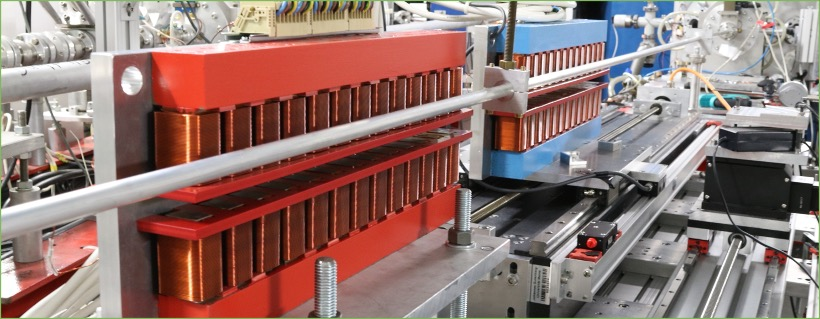
\includegraphics[width=0.8\linewidth]{image/1-1.jpg}\\
  \caption{サンプルの図}
  \label{optics_schematic}
\end{figure}
図\ref{optics_schematic}に光学系の概要を示す。
矩形スリットで整形した光波は伝搬に伴って回折を生じる\ref{sec:rayleigh}章。後段には回折格子およびレンズがあり、
光波は分光と平面波化\ref{sec:grating},\ref{sec:grating2}章を受けカメラに到達する。
\subsection{レイリー・ゾンマーフェルト回折積分}\label{sec:rayleigh}
光波の伝搬はマクスウェル方程式に従う。
ある平面の波面から別の平面での波面を計算するには、レイリーゾンマーフェルト回折積分が知られている。
今回のセットアップにおいては近軸近似を用いることで、スクリーンでの回折パターンを式(??)によって計算できる。
回折現象は以下のレイリーゾンマーフェルト積分によって厳密に計算することができる
\begin{eqnarray}
  \text{U}(\text{P}) = \frac{1}{4\pi}\int_{S}\cos(ns)\text{U}(S)\frac{\exp(iks)}{s}\left( ik - \frac{1}{s}\right) -U(S)\frac{\exp(iks)}{s}\left(ik- \frac{1}{r}\right)\cos(nr) dS
\label{レイリーゾンマーフェルト}
\end{eqnarray}
近似① $k \gg 1/r$, $k \gg 1/s$
近似② $\cos(nr) \sim 1$,$\cos(ns) \sim 1$
近似③ 領域Sにおいて$r(S)= z = \text{const.}$,$s(S) = s_0 = \text{const.}$
により式(\ref{レイリーゾンマーフェルト})は
\begin{eqnarray}
  \text{U}(P) = -\frac{i}{2\lambda rs} \int_{S} U(S)\exp ik(r+s) dS
  \label{レイリーゾンマーフェルト近似}
\end{eqnarray}
\begin{eqnarray}
  \text{U}(P) = -\frac{i}{2\lambda rs} \int_{S} U(S)\exp ikr dS
\end{eqnarray}
このような回折現象は伝搬距離によっては近似計算できることが知られている。以下では積分領域$S$上の座標を$x,y$、観測点Pの座標を$x_0,y_0$と表記する。
\begin{eqnarray}
  r &=& \sqrt{z^2 + (x-x_0)^2 + (y-y_0)^2}\\
  &=& z + \frac{1}{2}\frac{(x-x_0)^2 + (y-y_0)^2}{z} - \frac{1}{8}\frac{\left[(x-x_0)^2 + (y-y_0)^2\right]^2}{z^3} +\dots
\end{eqnarray}
$\left[(x-x_0)^2 + (y-y_0)^2\right]^2 \ll z^3$が成立するなら
\begin{eqnarray}
  \text{U}(x_0,y_0) \sim -\frac{i}{2\lambda zs_0}\int \text(U)(x,y) \exp(ik\left\{z +\frac{1}{2}\frac{(x-x_0)^2 + (y-y_0)^2}{z}\right\})
\end{eqnarray}

数値計算手法については第3章に記述する。
\subsection{回折格子とレンズによる分光}\label{sec:grating}
波面は回折格子で波長ごとに特定の方向に分光される。
レンズによって集光することでカメラでは特定の波長が鋭いピークとなるため、高い波長分解能を実現できる。
\subsection{回折格子による平面波化}\label{sec:grating2}
回折格子は図(??)のようにブレードと呼ばれる溝が掘られている。
光波はブレードによって反射されるが、隣り合うブレードから反射される光波は干渉を起こし、平面波となる。
このような平面波化はフーリエ変換として理解できる。
タンデム型アンジュレータから放射されるダブルパルス型の放射光が回折格子によって平面波化されることで、前後のパルスが干渉を起こす。
\subsection{電子ビームの集団運動}
これまでの議論は電子1個の場合について述べたが、実際には電子ビームは多数の電子からなり、放射光もその一つ一つから放射されるパルスの重ね合わせである。
そのため、異なる電子から放射されたパルス同士が干渉することも考慮しなければいけないが、自己相関の干渉項以外はランダム性から無視できると考えられる。
\subsection{撮影画像}
これらの一連の流れを図(??)に示した。
放射光がスリットによって回折を受けると、カメラでは2次元の回折パターン構造が得られると推定される。
一方で回折格子による分光、平面波化作用は水平方向にのみ作用する。従って画像の横軸は波長に対応し、縦軸の座標は観測角に対応する。
\subsection{モデル関数}
モデル関数の概要を示す。
アンジュレータの位置とカメラにおけるy座標の関数として定義される。
放射光関数は、電子ビームとアンジュレータのパラメータを入力としてスリット直前の入射光の振幅および位相を計算する。
光学関数は、入射光の位相と振幅を入力としてスクリーンにおける回折光の振幅を計算する。

撮影画像を再現する最も確からしいパラメータの組を求めることで、電子ビームのエネルギーが決定できる。
\end{document}

\documentclass[a4paper,11pt,uplatex]{jsbook}
%\usepackage{fancyhdr}
\setlength{\footskip}{16pt}
\usepackage{amsmath}
\usepackage[dvipdfmx]{graphicx}
\usepackage[dvipdfmx]{color}
%\usepackage{pagecolor}[white]
\usepackage{amsmath,amssymb}
%\usepackage[top=3cm, bottom=3cm, left=3cm, right=3cm]{geometry}
\usepackage{braket}
\usepackage{bm}
\numberwithin{equation}{section}
\usepackage{mathrsfs}
\usepackage{siunitx}
\usepackage{physics}
\usepackage[dvipdfmx]{graphicx}
\usepackage[compat=1.1.0]{tikz-feynhand}
\usepackage{caption}
\usepackage{subcaption}
%\usepackage{cleveref}
\usepackage{float}
\usepackage{multicol}
\setlength{\columnsep}{15mm}
%\usepackage[style=phys,articletitle=false,biblabel=brackets,chaptertitle=false,pageranges=false]{biblatex}
%\usepackage[style=phys]{biblatex}
\usepackage[dvipdfmx]{hyperref}
\usepackage{url}
\usepackage{pxjahyper}
\usepackage{bookmark}
%\usepackage[backref]{hyperref}
\setcounter{tocdepth}{3}
\setlength{\parindent}{2em}
\def\vector#1{\mbox{\boldmath $#1$}}
\def\slash#1{\not\!#1}
\def\slashb#1{\not\!\!#1}
\def\delsla{\not\!\partial}
%\usepackage[dvipdfmx]{xcolor}


\hypersetup{
 setpagesize=false,
 bookmarksnumbered=true,%
 bookmarksopen=true,%
 colorlinks=true,%
 linkcolor=black,
 citecolor=red,
 urlcolor=black,
}
%backreferenceのカスタマイズ. "Back to p.3"のように表示する.
%\renewcommand*{\backref}[1]{(p.#1へ戻る)}
%\newcommand{\backtoc}{\hyperlink{toc}{[目次へ]}}
\newcommand{\backtoc}{\texorpdfstring{\protect\hyperlink{toc}{\hspace{5pt} \scriptsize [目次へ]}}{}}
\newcommand{\mychapter}[1]{\chapter[#1]{#1\backtoc}}
\newcommand{\mysection}[1]{\section[#1]{#1\backtoc}}
\newcommand{\mysubsection}[1]{\subsection[#1]{#1\backtoc}}

% 数式
%\usepackage{amsmath,amsfonts}
%\usepackage{bm}
%\usepackage{physics}
% 画像
%\usepackage[dvipdfmx]{graphicx}
%\usepackage[dvipdfmx,colorlinks=true,linkcolor=blue]{hyperref}
%\usepackage{pxjahyper}

\begin{document}


\chapter{MAMIにおける測定手法}
この章の目的は、実験に用いた装置の性能や仕様、およびセットアップの手法を説明することである。
まず加速器とMAMIの概要を示し、高品質のアンジュレータ放射光を得るための制御方法を説明する。
次に、電子ビームエネルギー測定に不可欠な分光光学系の構成とアラインメント方法を示す。
最後に、ビームタイム中のデータ取得の手順を示す。
\section{装置とセットアップ}
\subsection{マインツマイクロトロン(MAMI)}\label{sec:MAMI}
MAinz MIcrotron~(MAMI)はドイツ、マインツ大学が所有する連続電子線加速器施設である。最大エネルギー1508 MeVの電子ビームを供給する
3台のRTM(Race Track Microtron)および1台のHDSM(Harmonic Double Sided Micrtron)から構成される。
MAMIのフロアマップを図\ref{fig:MAMI}に、主なパラメータを表\ref{MAMI}に示した。
ハイパー核生成実験ではHDSMを用いて最大エネルギーの1508 MeVの電子ビームを供給する。

スペクトロメータ較正実験では、RTM3までで加速された180 MeVから210 MeVまでの電子ビームを用いる。
\begin{figure}[H]
  \centering
  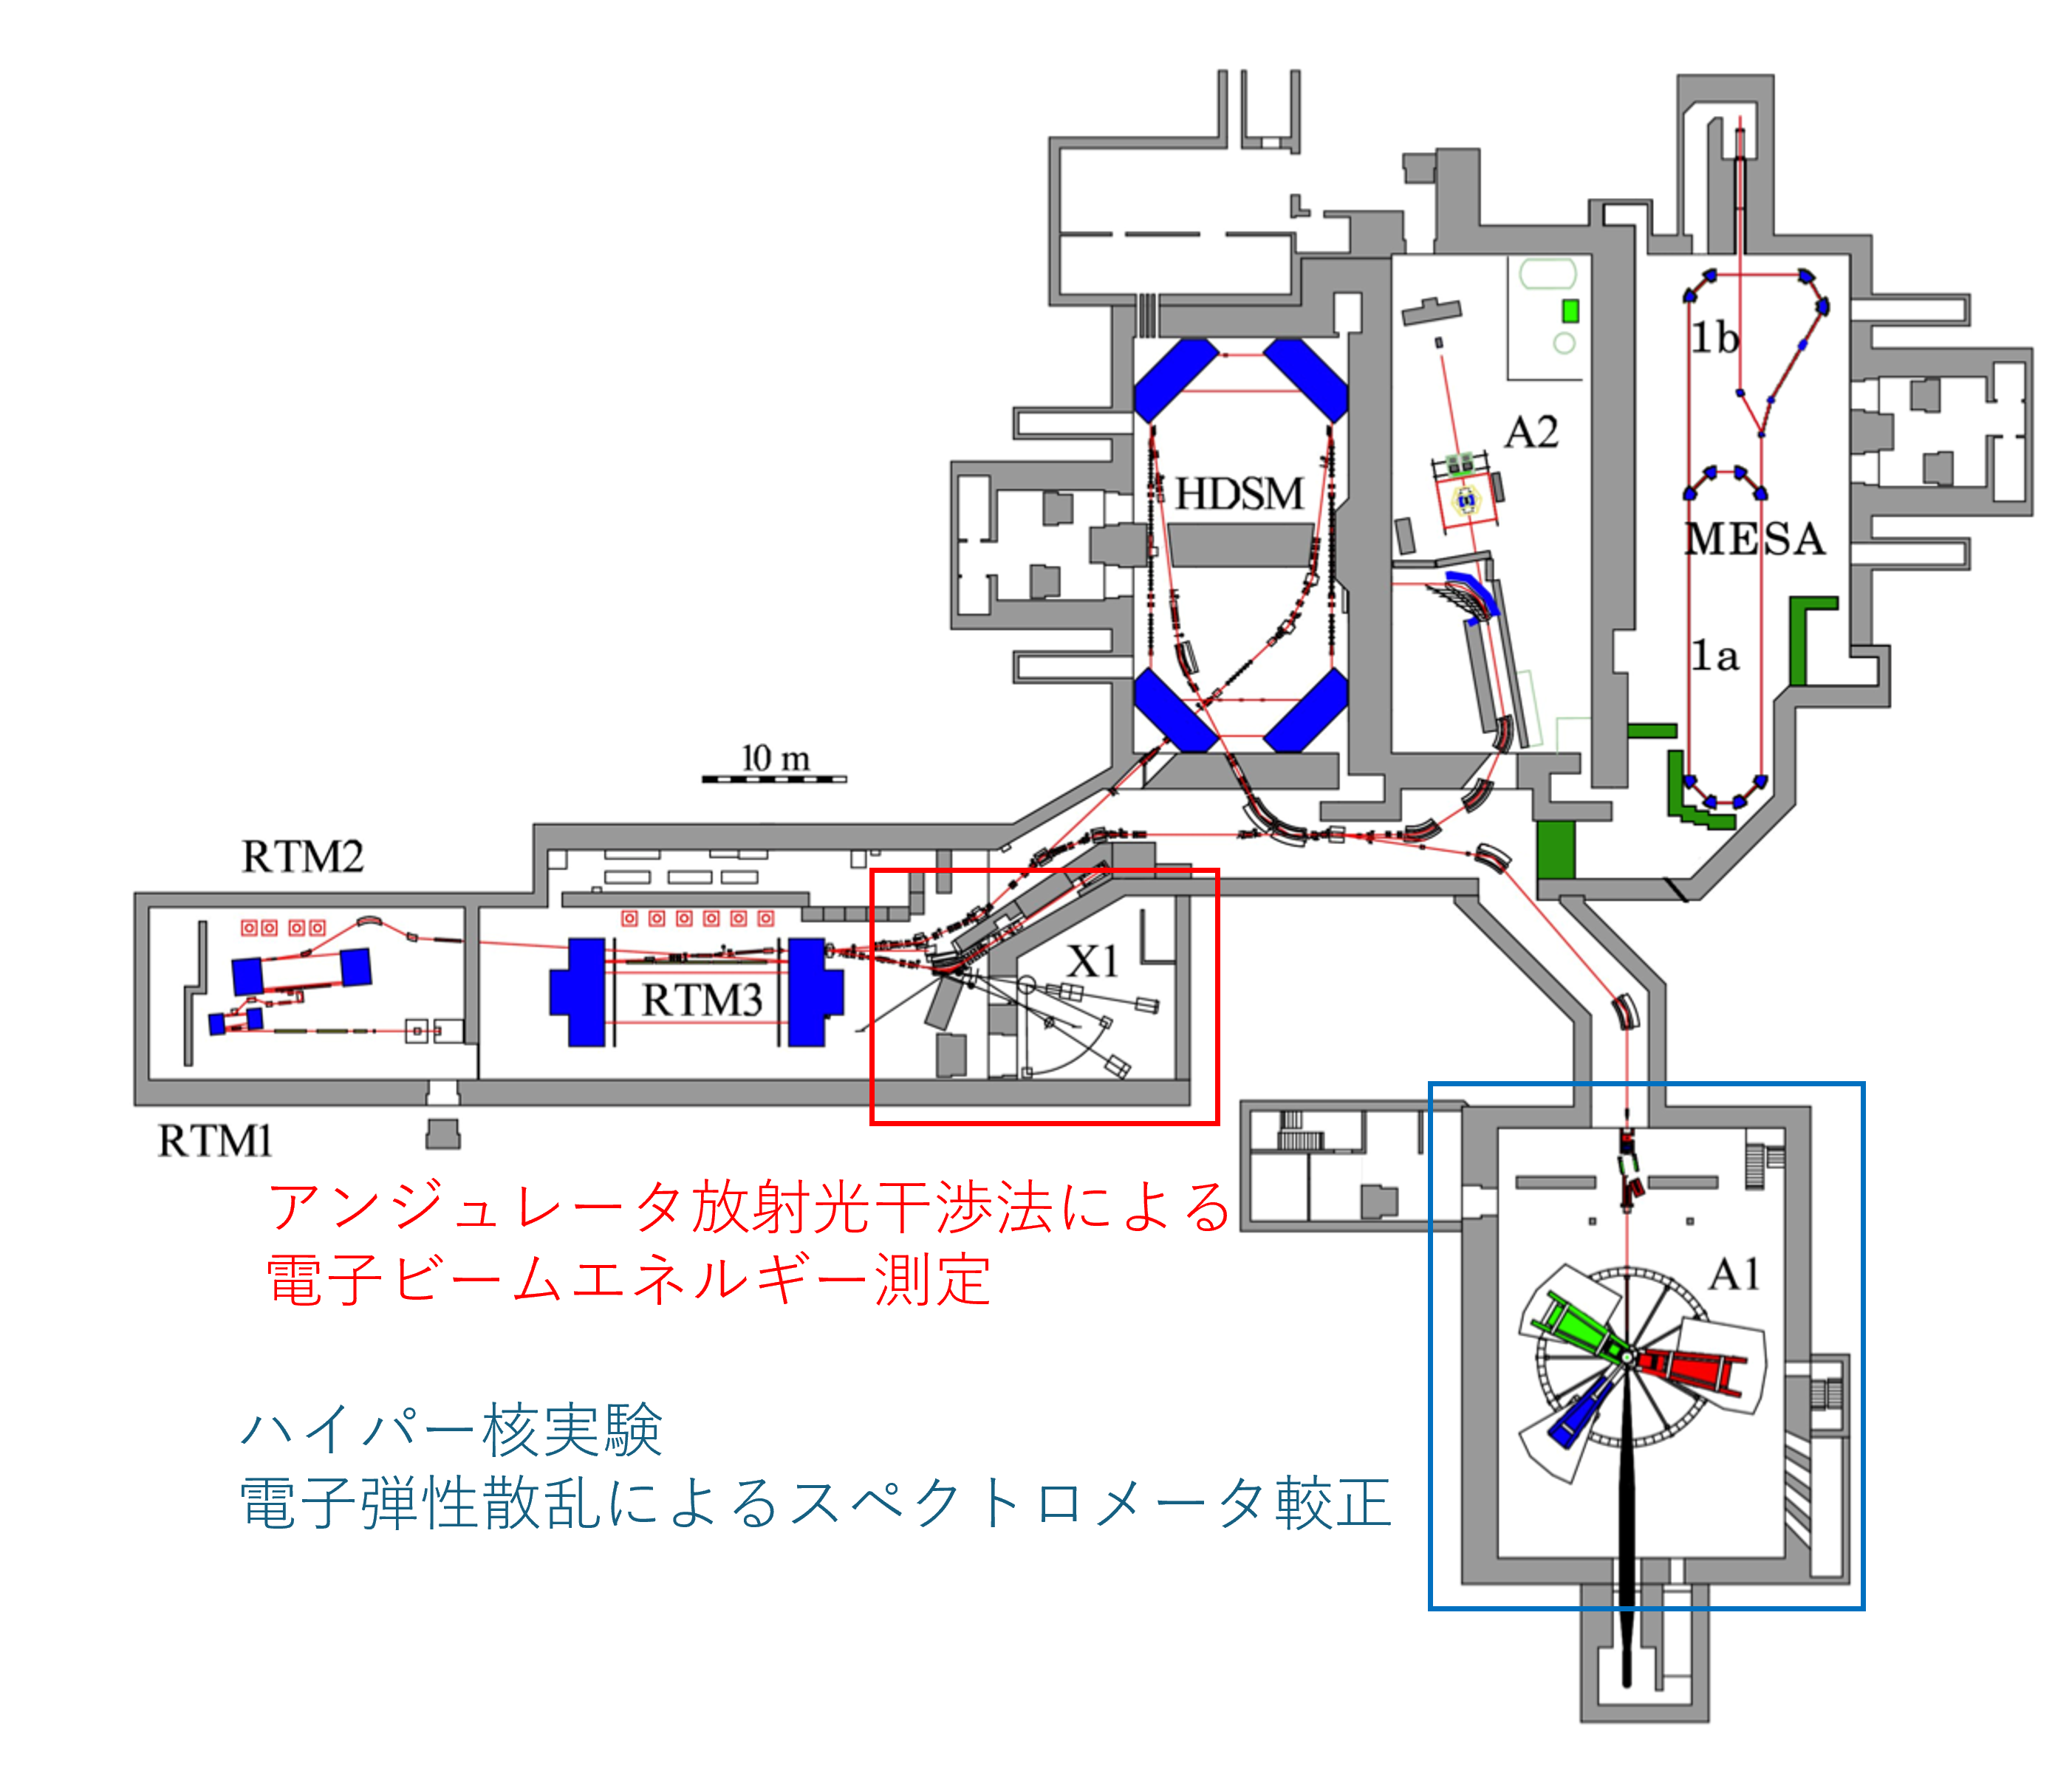
\includegraphics[width=0.8\linewidth]{image/3-MAMI.png}\\
  \caption[MAMIのフロアマップ]{MAMIのフロアマップ。RTM1,RTM2,RTM3で加速された電子ビームはX1ホール(赤)またはA1ホール(青)に供給される。X1ホールではアンジュレータ放射光干渉法による電子ビームエネルギー測定を行う。またA1ホールでは電子弾性散乱実験を行う。}
  \label{fig:MAMI}
\end{figure}
\begin{table}[H]
  \caption{MAMIの主要パラメータ}\label{MAMI}
  \centering
  \begin{tabular}{c||cc}
    \hline
     &RTM3 & HDSM \\
    \hline
    最大エネルギー & 855.1 MeV & 1508 MeV \\
    最大強度 & 100 $\mu$A & 100 $\mu$A \\
    周回数 & 90 & 43 \\
    偏光磁石の磁場 &1.28 T & 0.95 - 1.53 T\\
    周波数 & 2.45 GHz & 2.45 / 4.9 GHz \\
    エネルギー幅 & 13 keV & 110 keV \\
    水平方向エミッタンス & 13 $\pi$ $\mu$m mrad & 27 $\pi$ $\mu$m mrad \\
    垂直方向エミッタンス & 0.84 $\pi$ $\mu$m mrad & 1.2 $\pi$ $\mu$m mrad\\
    \hline
  \end{tabular}
\end{table}
ここでは本研究で用いる200 MeV領域の電子ビームに注目し、RTM3における加速機構を説明する。
図\ref{RTM3}にRTM3の模式図を示した。2つの180$^\circ$偏向電磁石の間には線形加速器(LINAC)が設置されている。
前段の加速器で180 MeVまで加速され入射された電子はLINACで加速されるごとにおよそ15 MeVエネルギーを得る。加速されると偏向電磁石での軌道半径が大きくなり、
一つ外側の周回軌道を通り再びLINACで加速を受ける。このようにして電子は周回軌道を繰り返し、最終的に最大で855 MeVまで加速されて実験ホールに供給される。
周回軌道の途中にはビーム取り出しのためのキッカーマグネットが設置されており、このキッカーマグネットをどの軌道に設置するかによって周回回数を調節し、供給するエネルギーを決定する。
\begin{figure}[h]
  \centering
  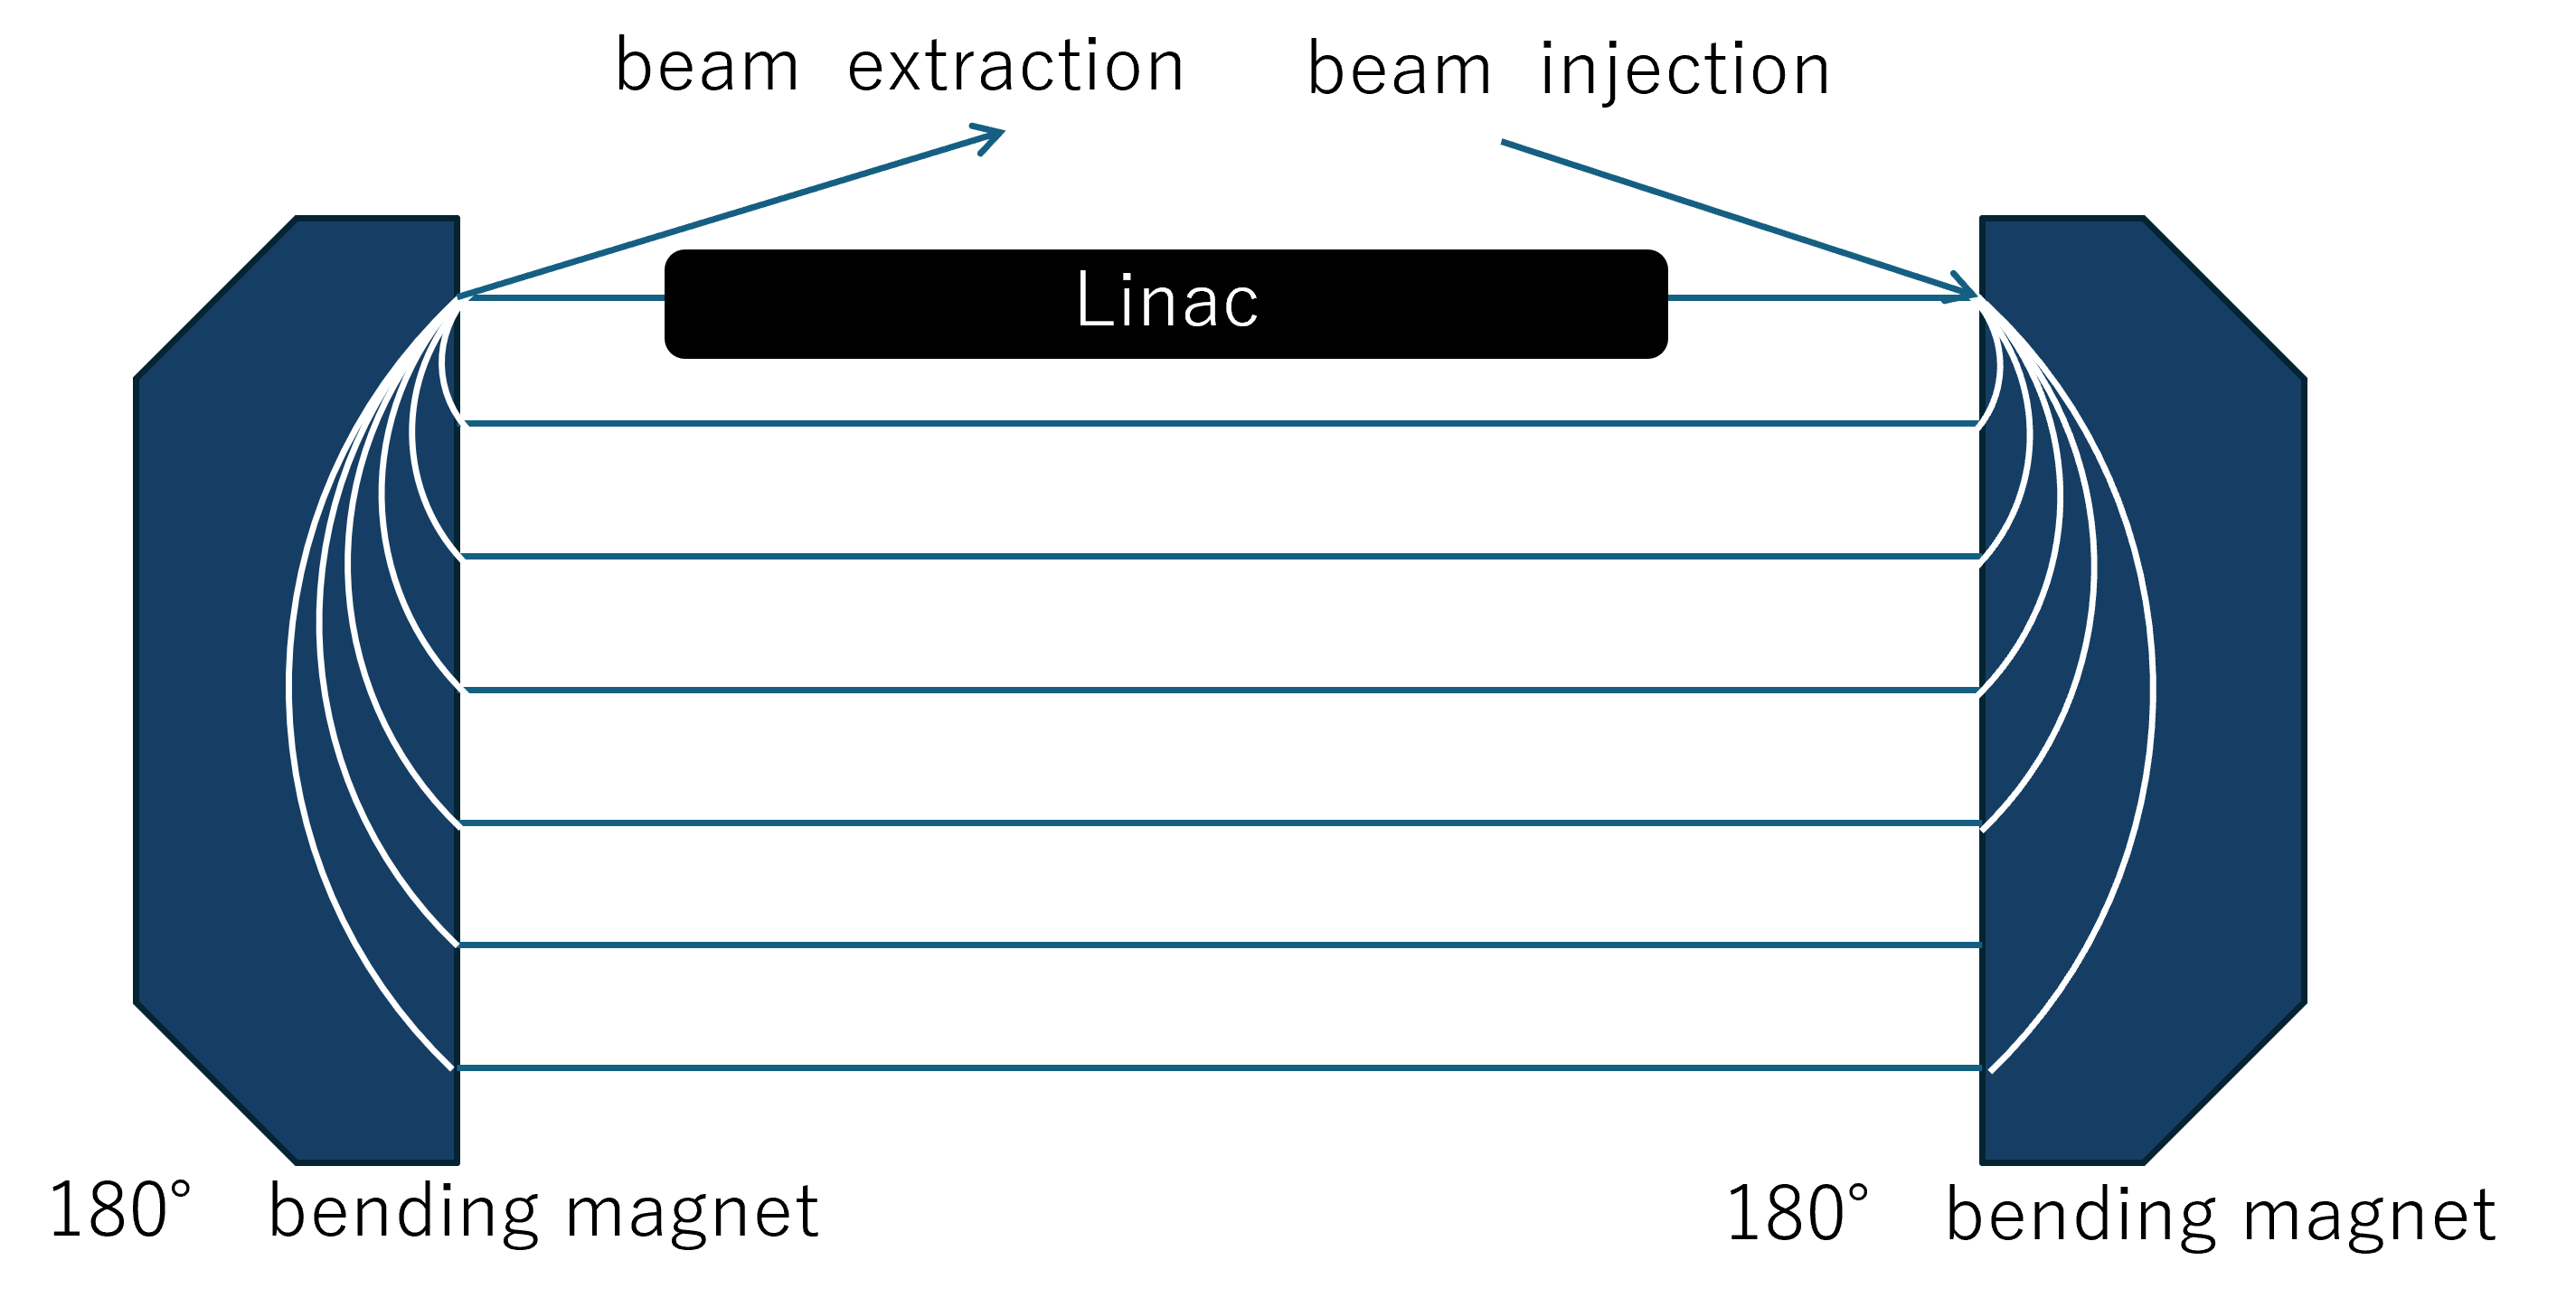
\includegraphics[width=0.8\linewidth]{image/3-RTM.png}\\
  \caption[RTM3の模式図]{RTM3の模式図。前段のRTM2で180 MeVまで加速された電子ビームは180$^\circ$偏向電磁石でもっとも軌道半径の小さい周回軌道に入る。
  1周してLINACで加速されるごとに15 MeVずつエネルギーが増加し、これに伴い軌道半径が大きくなり、一つ外側の周回軌道を通り再びLINACで加速を受ける。
  軌道中に設置したキッカーマグネットによって周回軌道からずれビーム取り出しビームラインに供給される。}
  \label{RTM3}
\end{figure}

RTM3には計90周の周回軌道があり、1周毎に15~MeVずつ加速されるが、このうち73週目の軌道にビームポジションモニタが設置されている。
RTM3の180$^\circ$偏向電磁石中での軌道半径$R_{73}$を測定し、得られたビームエネルギー$E_{73}$からMAMIで確立された粒子トラッキングシステムPTRACE\cite{ratschow}を用いて$n$周目のビームエネルギー$E_n$を外挿して求める。
180$^\circ$偏向電磁石の磁場はNMRを用いて$10^{-4}$の精度で測定されている。またPTRACEの計算で生じる誤差が0.1~mm、ビームパイプの位置決定精度が0.43~mmと見積もられており、
これらの誤差を考慮して$E_{73}\sim 727~$MeVにおけるエネルギーの誤差は$\delta E_{73} =120$~keVと見積もられている\cite{jankowiak}。
$E_{73}$から他の周回軌道のビームエネルギー$E_n$をPTRACEで外挿した結果、$E_n$の誤差は一律で$\delta E_n$ =160~keVと見積もられている\cite{herter}。

RTM3の直後には供給するビームラインを選ぶための偏向電磁石が設置されており極性をレバーで変えることで、アンジュレータ放射光干渉法による電子ビームエネルギー測定を行うX1ホールと、電子弾性散乱によるスペクトロメータ較正を行うA1ホールにビームを供給するモードを切り替えることができる。

\subsubsection{X1ホール}
電子ビームエネルギー測定を行うホールBとX1ホールの構成を図\ref{X1}, \ref{X1-2}に示す。
\begin{figure}[H]
  \centering
  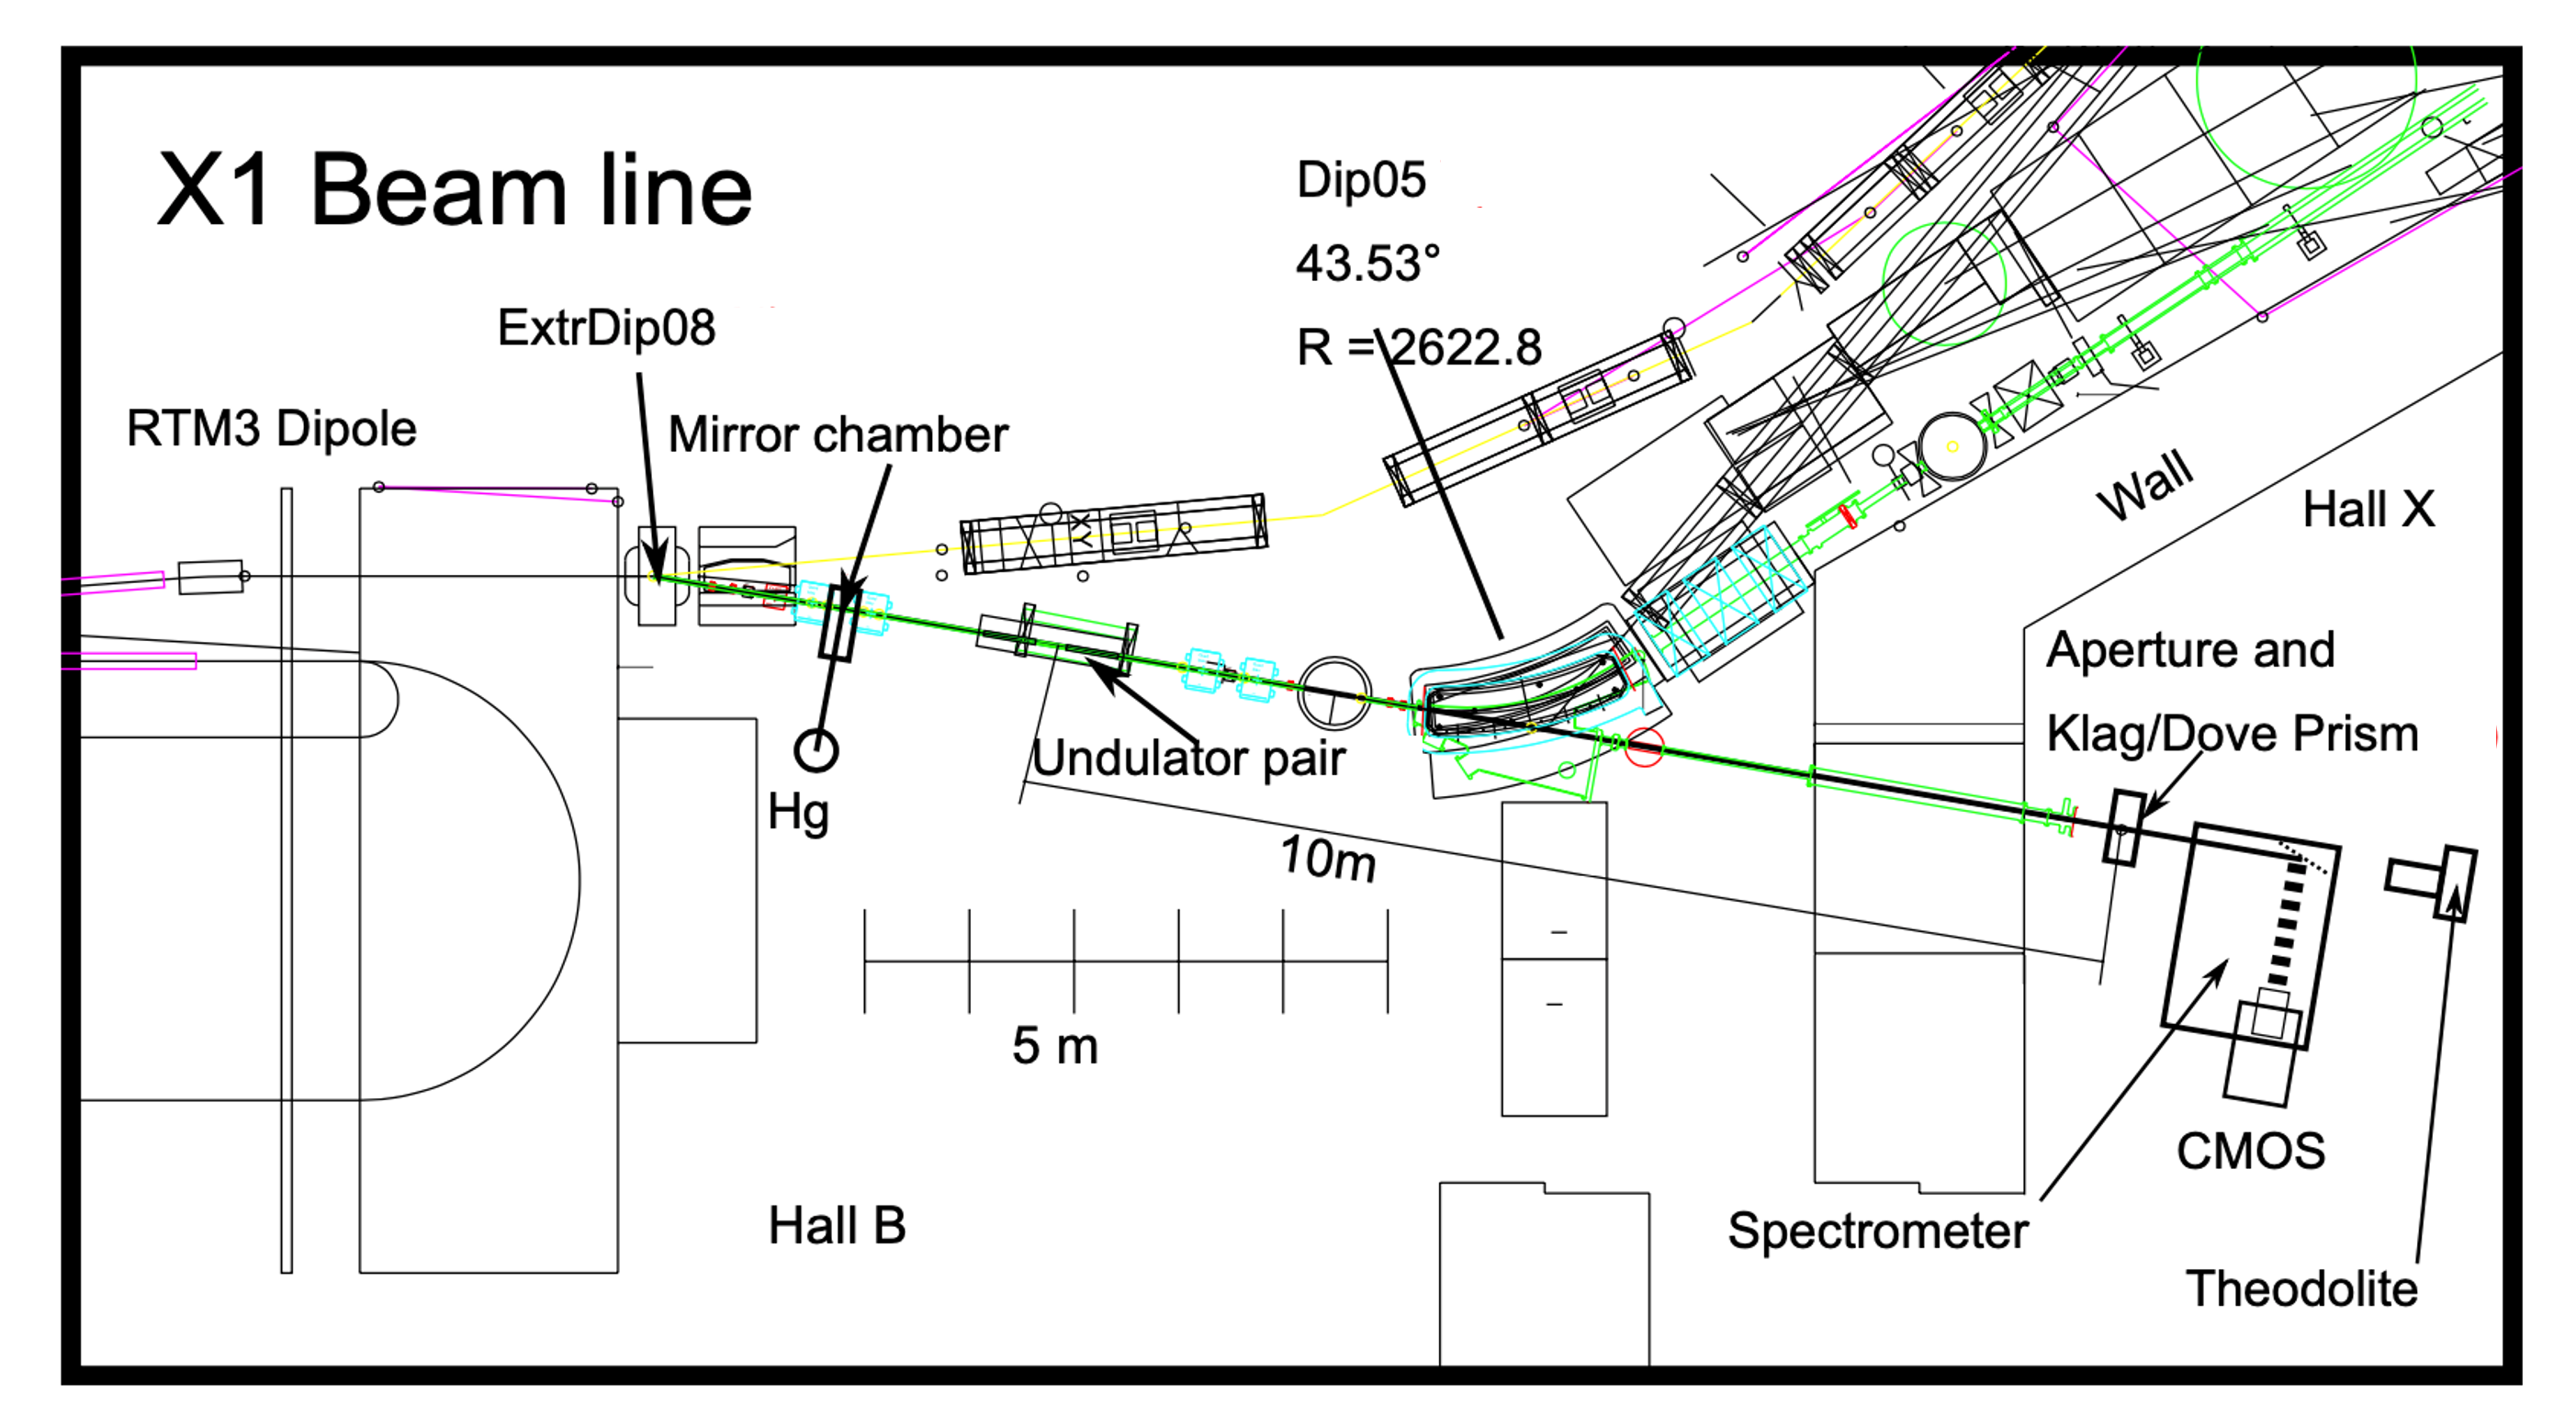
\includegraphics[width=\linewidth]{image/3-X1.png}\\
  \caption[ホールBとX1ホールの模式図]{ホールBとX1ホールの模式図。電子ビームは図の左のRTM3側から供給される。RTM3偏向電磁石の直後にある一つ目の偏向電磁石では電子ビームを供給するビームラインを選択する。
  電子ビームエネルギー測定をおこなうときには電子ビームは図の下側のビームラインへ供給される。四重極電磁石(Q1,Q2)の間にはミラーボックスを設置し
  光学系の較正用のレーザー光をビームラインに導く。Q2の下流にアンジュレータを設置し、ここで放射光を発生させる。アンジュレータの下流には更に2つの四重極電磁石Q3,Q4、および偏向電磁石が設置されている。
  偏向電磁石によって電子ビームはビームダンプへ導かれ、放射光のみを観測する光学系に導くことができる。コンクリート壁を隔ててX1ホールに光学系を設置し放射光のデータ取得を行うほか、更に下流にはアラインメント用のセオドライトを設置する}
  \label{X1}
\end{figure}
\begin{figure}[H]
  \centering
  \includegraphics[width=\linewidth]{image/3-HallB.png}\\
  \caption[ホールBの写真]{ホールBのビームラインを上から撮影した画像。図\ref{X1}の模式図のQ1からビームダンプへの偏向電磁石までが見えている。}
  \label{X1-2}
\end{figure}
電子ビームの軌道を調整するための電磁石がRTM3に設置されており、水平方向、垂直方向のビーム位置を調整する。
RTMの直後にはビームライン選択用の偏向電磁石が設置されている。更に下流には四重極電磁石が2つ(Q1,Q2)設置されており、その間にミラーボックスが設置されている。
Q2の下流にアンジュレータを2台設置する。その下流に更に2台の四重極電磁石(Q3,Q4)が設置されている。
4台の四重極電磁石はアラインメントの基準となるほか、ビーム調整時にも利用するが、測定を行う際には原則利用しない。
その下流には偏向電磁石が設置されており、電子ビームをビームダンプに導くことができる。これにより放射光のみをコンクリート壁に通したビームパイプを通じてX1ホールに導くことができる。
X1ホールには光学系が設置されており、放射光を観測する。アンジュレータから光学系まではおよそ10 mの距離がある。更にその下流側にはアラインメント用のセオドライトが設置されている。

またホールBのビームライン上には光学系の較正用の水銀灯や青色レーザー、ビームライン内の可動式ミラーが設置されている。
水銀灯や青色レーザーによる較正を行う際にはミラーボックス内のミラーをビームライン中心に移動させることで水銀灯や青色レーザーを光学系に供給することができる。
\begin{figure}[H]
  \centering
  \includegraphics[width=0.5\linewidth]{image/3-mirrorbox.png}\\
  \caption[ミラーボックスの写真]{ホールB内に設置されたミラーボックスを真上から撮影した画像。ビームタイム中は蓋がされており、遠隔でモーターを駆動することで
  ミラーを移動させる。写真では電子ビームを供給するモードの状態になっており、電子軌道からミラーが外れている。
  水銀灯による較正を行う際にはミラーが電子軌道に挿入され、図の左から入射する水銀灯の光をビームラインに平行にX1ホールに供給できる}
  \label{mirrorbox}
\end{figure}
\subsubsection{ビーム調整}
まずルミノシティモニタを用いてフェイントビームの位置を目測で調整する。この時の精度は1~mm間隔のグリッドの1/10として100~$\mu$m と見積もられる。
\begin{figure}[H]
  \centering
  \includegraphics[width=0.6\linewidth]{image/3-beamtune.png}\\
  \caption[ルミノシティモニタ]{ルミノシティモニタでのフェイントビームの照射領域。このモニタでビーム位置を目測しながらビーム調整用の電磁石の電流値を調整する。グリッドの間隔は1~mmである。}
  \label{luminosity}
\end{figure}

続いて、ビーム強度を5 $\si{\mu}\text{A}$に上げつつホールB内の放射線モニターで測定される放射線レベルがMAMIの安全基準よりも低くなるように微調整を行う。
この時放射線レベルが安全基準よりも高くなることは、ビームがビームダンプまで輸送されるまでにビームパイプ中心から外れ、ビームラインの内壁にビームが当たってしまっていることを示す。
最後にカメラを用いて放射光を見ながらビームの位置を調整する。スリットに対してビーム中心がずれている場合には回折パターンが上下非対称になる。

\subsection{アンジュレータ}
アンジュレータは自作のコイルを用いて製作した。各コイル対が独立に制御可能な電磁石となっている。1台のアンジュレータに計13個のコイルが等間隔かつ極性が交互に配置されている。
上下のギャップは18~mmである。ギャップサイズは固定し、電磁石の電流を調整することで磁場調整を行う。全長が520~mmである(図\ref{undulator})。
\begin{figure}[H]
  \centering
  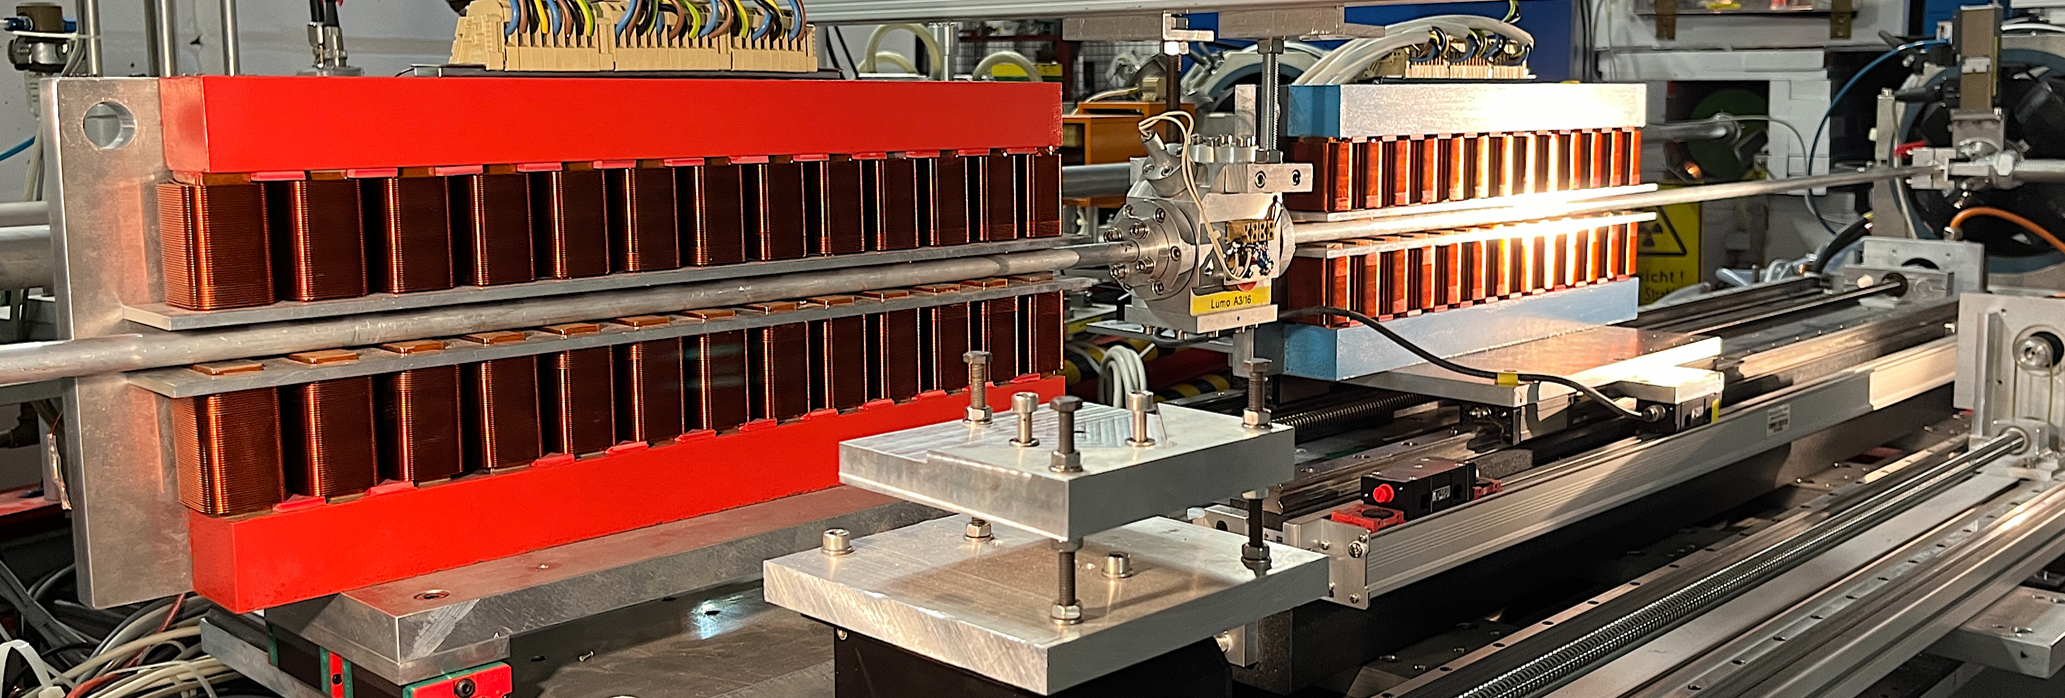
\includegraphics[width=\linewidth]{image/3-undulator.png}\\
  \caption[アンジュレータ]{測定に用いた2台のアンジュレータ。上流側の赤色アンジュレータは固定されているのに対し、、
  下流側の青色アンジュレータはステージに取り付けらえており、825 mmの可動範囲で$z$軸方向に移動できる。2台のアンジュレータの設計は同一で、
  13個のコイルが等間隔かつ極性が交互に配置されている。磁場1周期すなわちコイル2個分の長さは80 mmで、全長は520 mmである。
  図の手前には磁場調整の際に用いるホールプローブ取り付け台が設置されている。} 
  \label{undulator}
\end{figure}
\subsubsection{磁場制御}
各コイルには電源ボックスから電流を供給する。電流値を調整することで正弦波状の磁場を発生させることができる。
磁場の調整の際には、マトリックス型のホールプローブによる磁場測定を行う。
ホールプローブは40$\times$40 mm$^2$の領域に16$\times$16個、合計256個のホール素子を持ち、磁場の3次元成分を測定する(図\ref{hall})。
\begin{figure}[H]
  \centering
  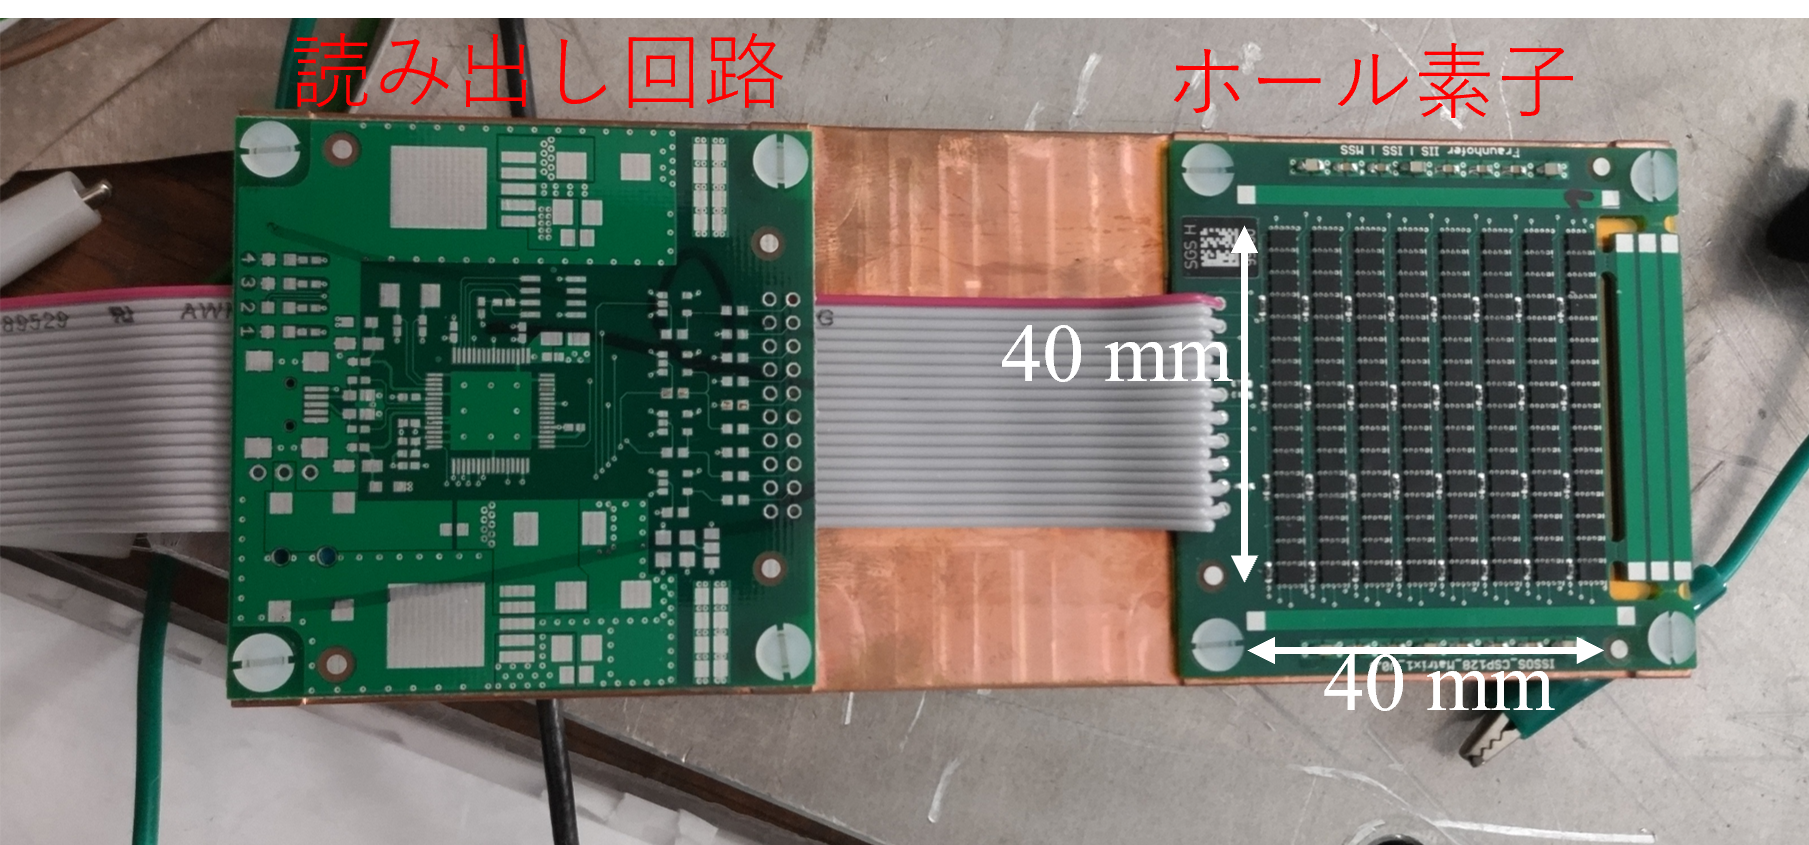
\includegraphics[width=0.7\linewidth]{image/3-hallmatrix.png}\\
  \caption[ホールプローブ]{マトリックス型のホールプローブ。40$\times$40 mm$^2$の領域に16$\times$16個、合計256個のホール素子を持ち、磁場の3次元成分を測定する。}
  \label{hall}
\end{figure}
ホールプローブはアンジュレータの中心を走査し磁場測定を行う。測定の様子を図\ref{hallscan}に示す。
\begin{figure}[H]
  \centering
  \includegraphics[width=0.8\linewidth]{image/3-HallMeasure.png}\\
  \caption[ホールプローブの走査]{ホールプローブによるアンジュレータの磁場測定の様子。ホールプローブはアンジュレータの中心を走査し、磁場の3次元成分を測定する。}
  \label{hallscan}
\end{figure}
アンジュレータ内の磁場は隣り合う複数の電磁石から影響を受けるため、適切な磁場を得るためには全ての電磁石の電流を同時に調整する必要がある。
ホールプローブによる測定と最適な電流値の決定を数回繰り返すことで、アンジュレータ内の磁場を調整する。
調整を止める基準として、アンジュレータを通過した後の電子軌道の変位が10~$\mu$m以下になることを定めて調整した。
調整後の磁場と、磁場の積分から計算される電子軌道の推定値を図\ref{fig:magnetic}に示す。
\begin{figure}[H]
  \centering
  \begin{subfigure}[h]{0.45\linewidth}
    \centering
    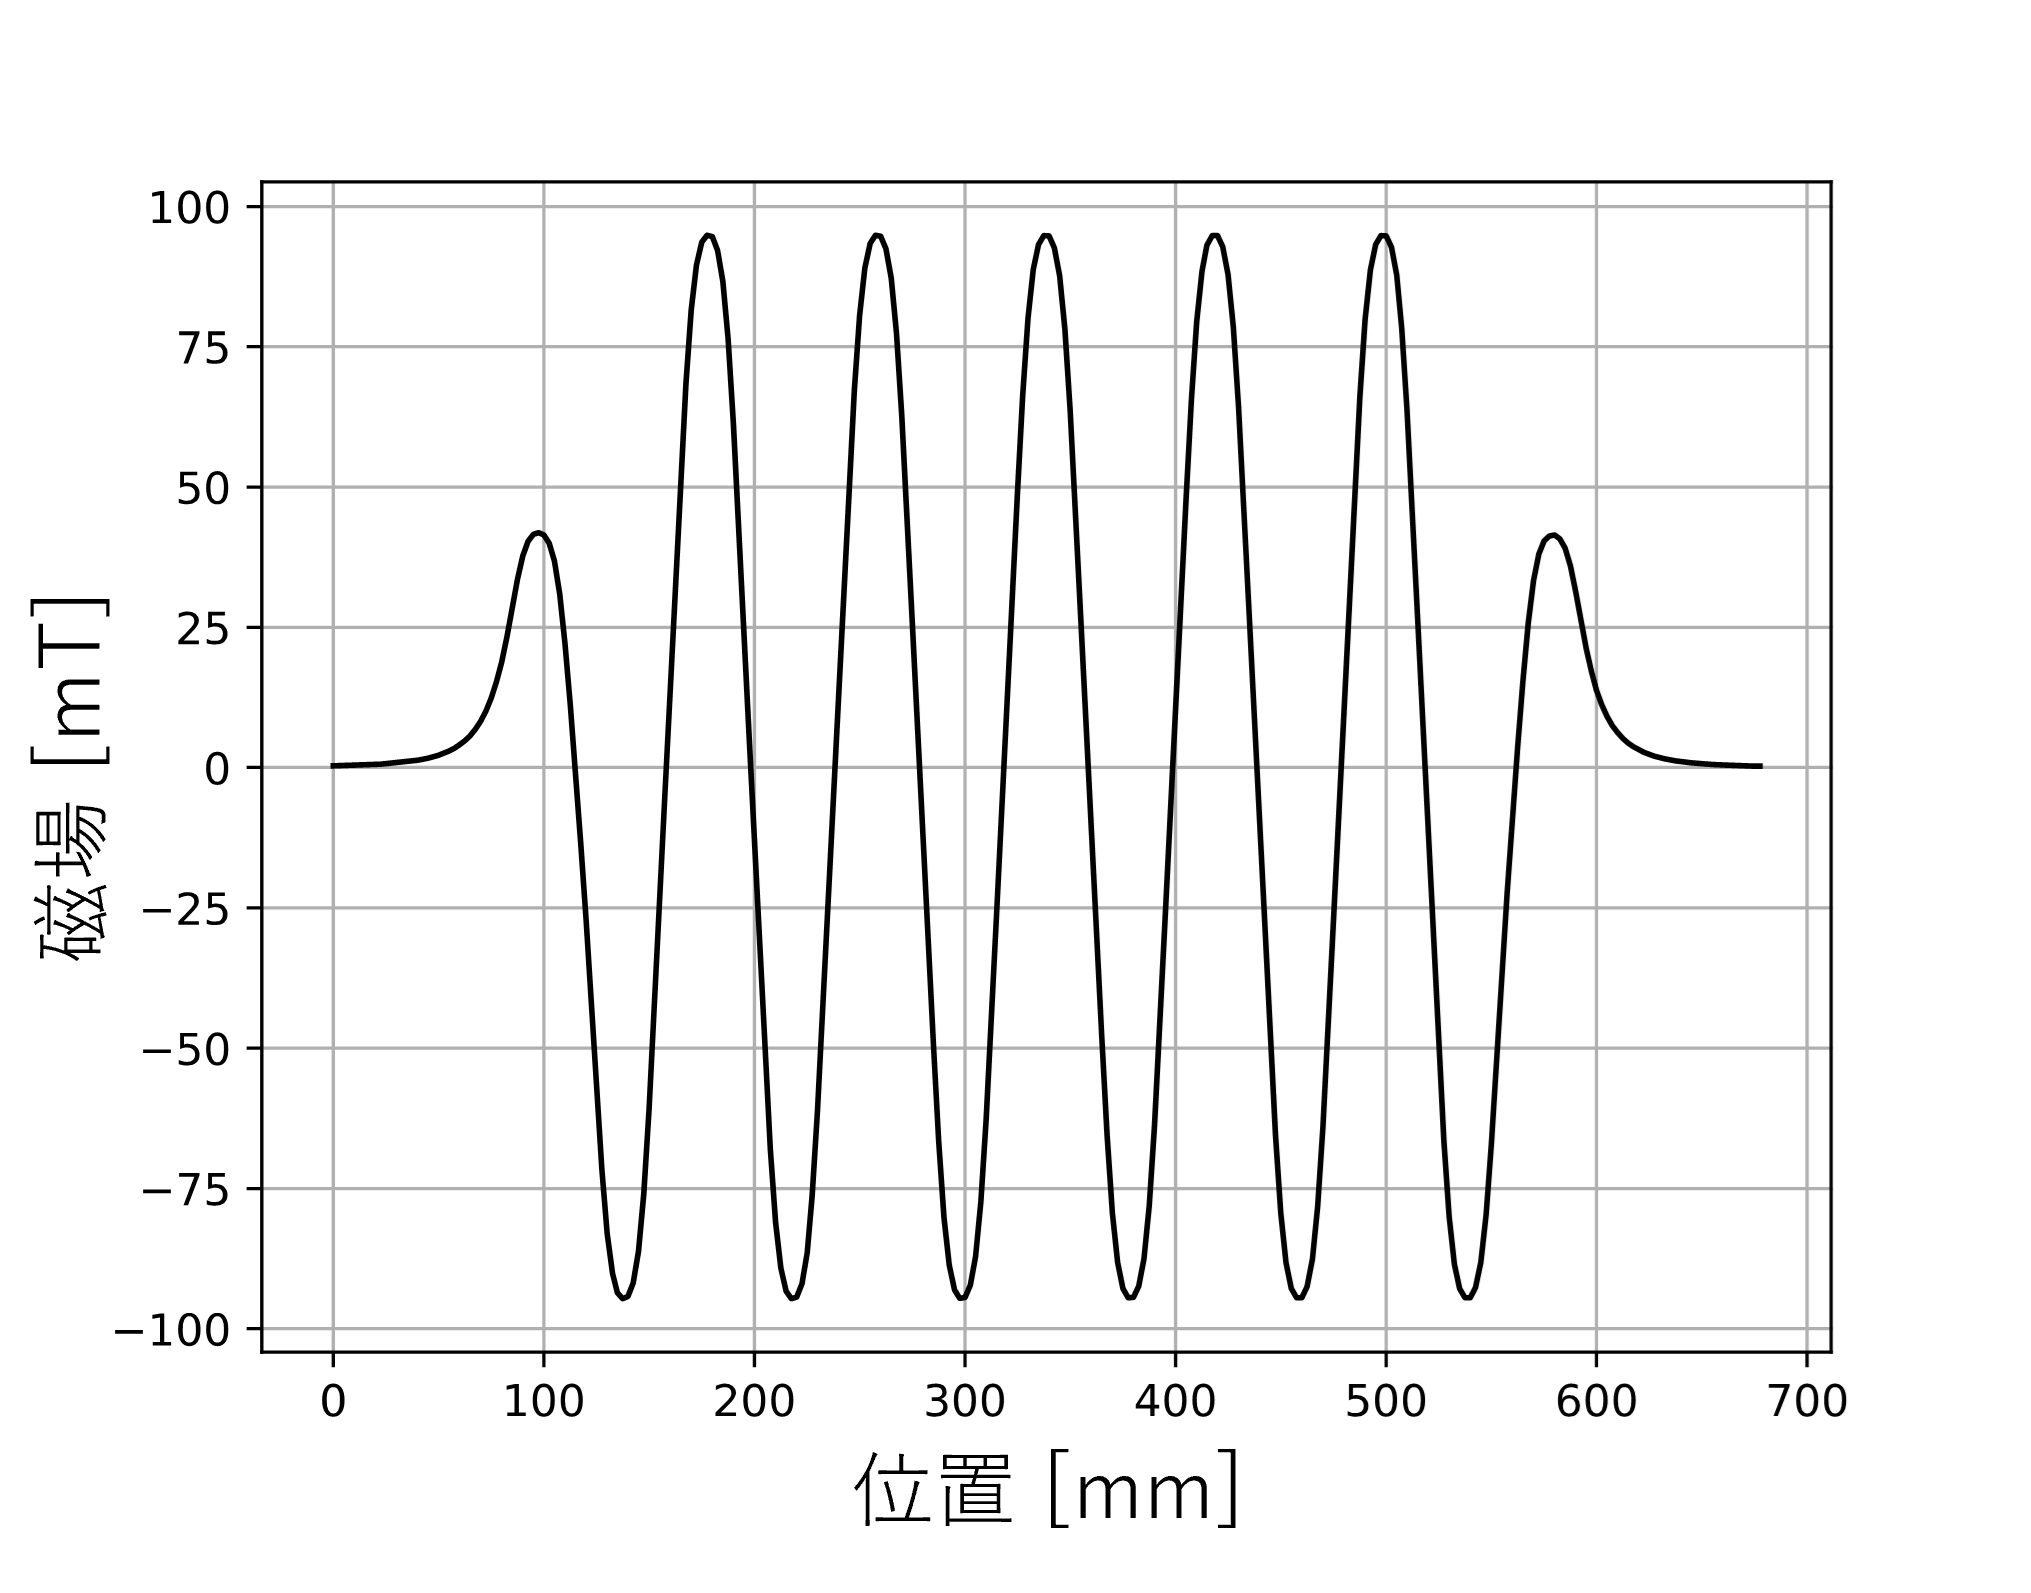
\includegraphics[width=\linewidth]{image/3-undulator_filed.png}
    \subcaption{磁場測定の結果}
  \end{subfigure}
  \hfill
  \begin{subfigure}[h]{0.45\linewidth}
    \centering
    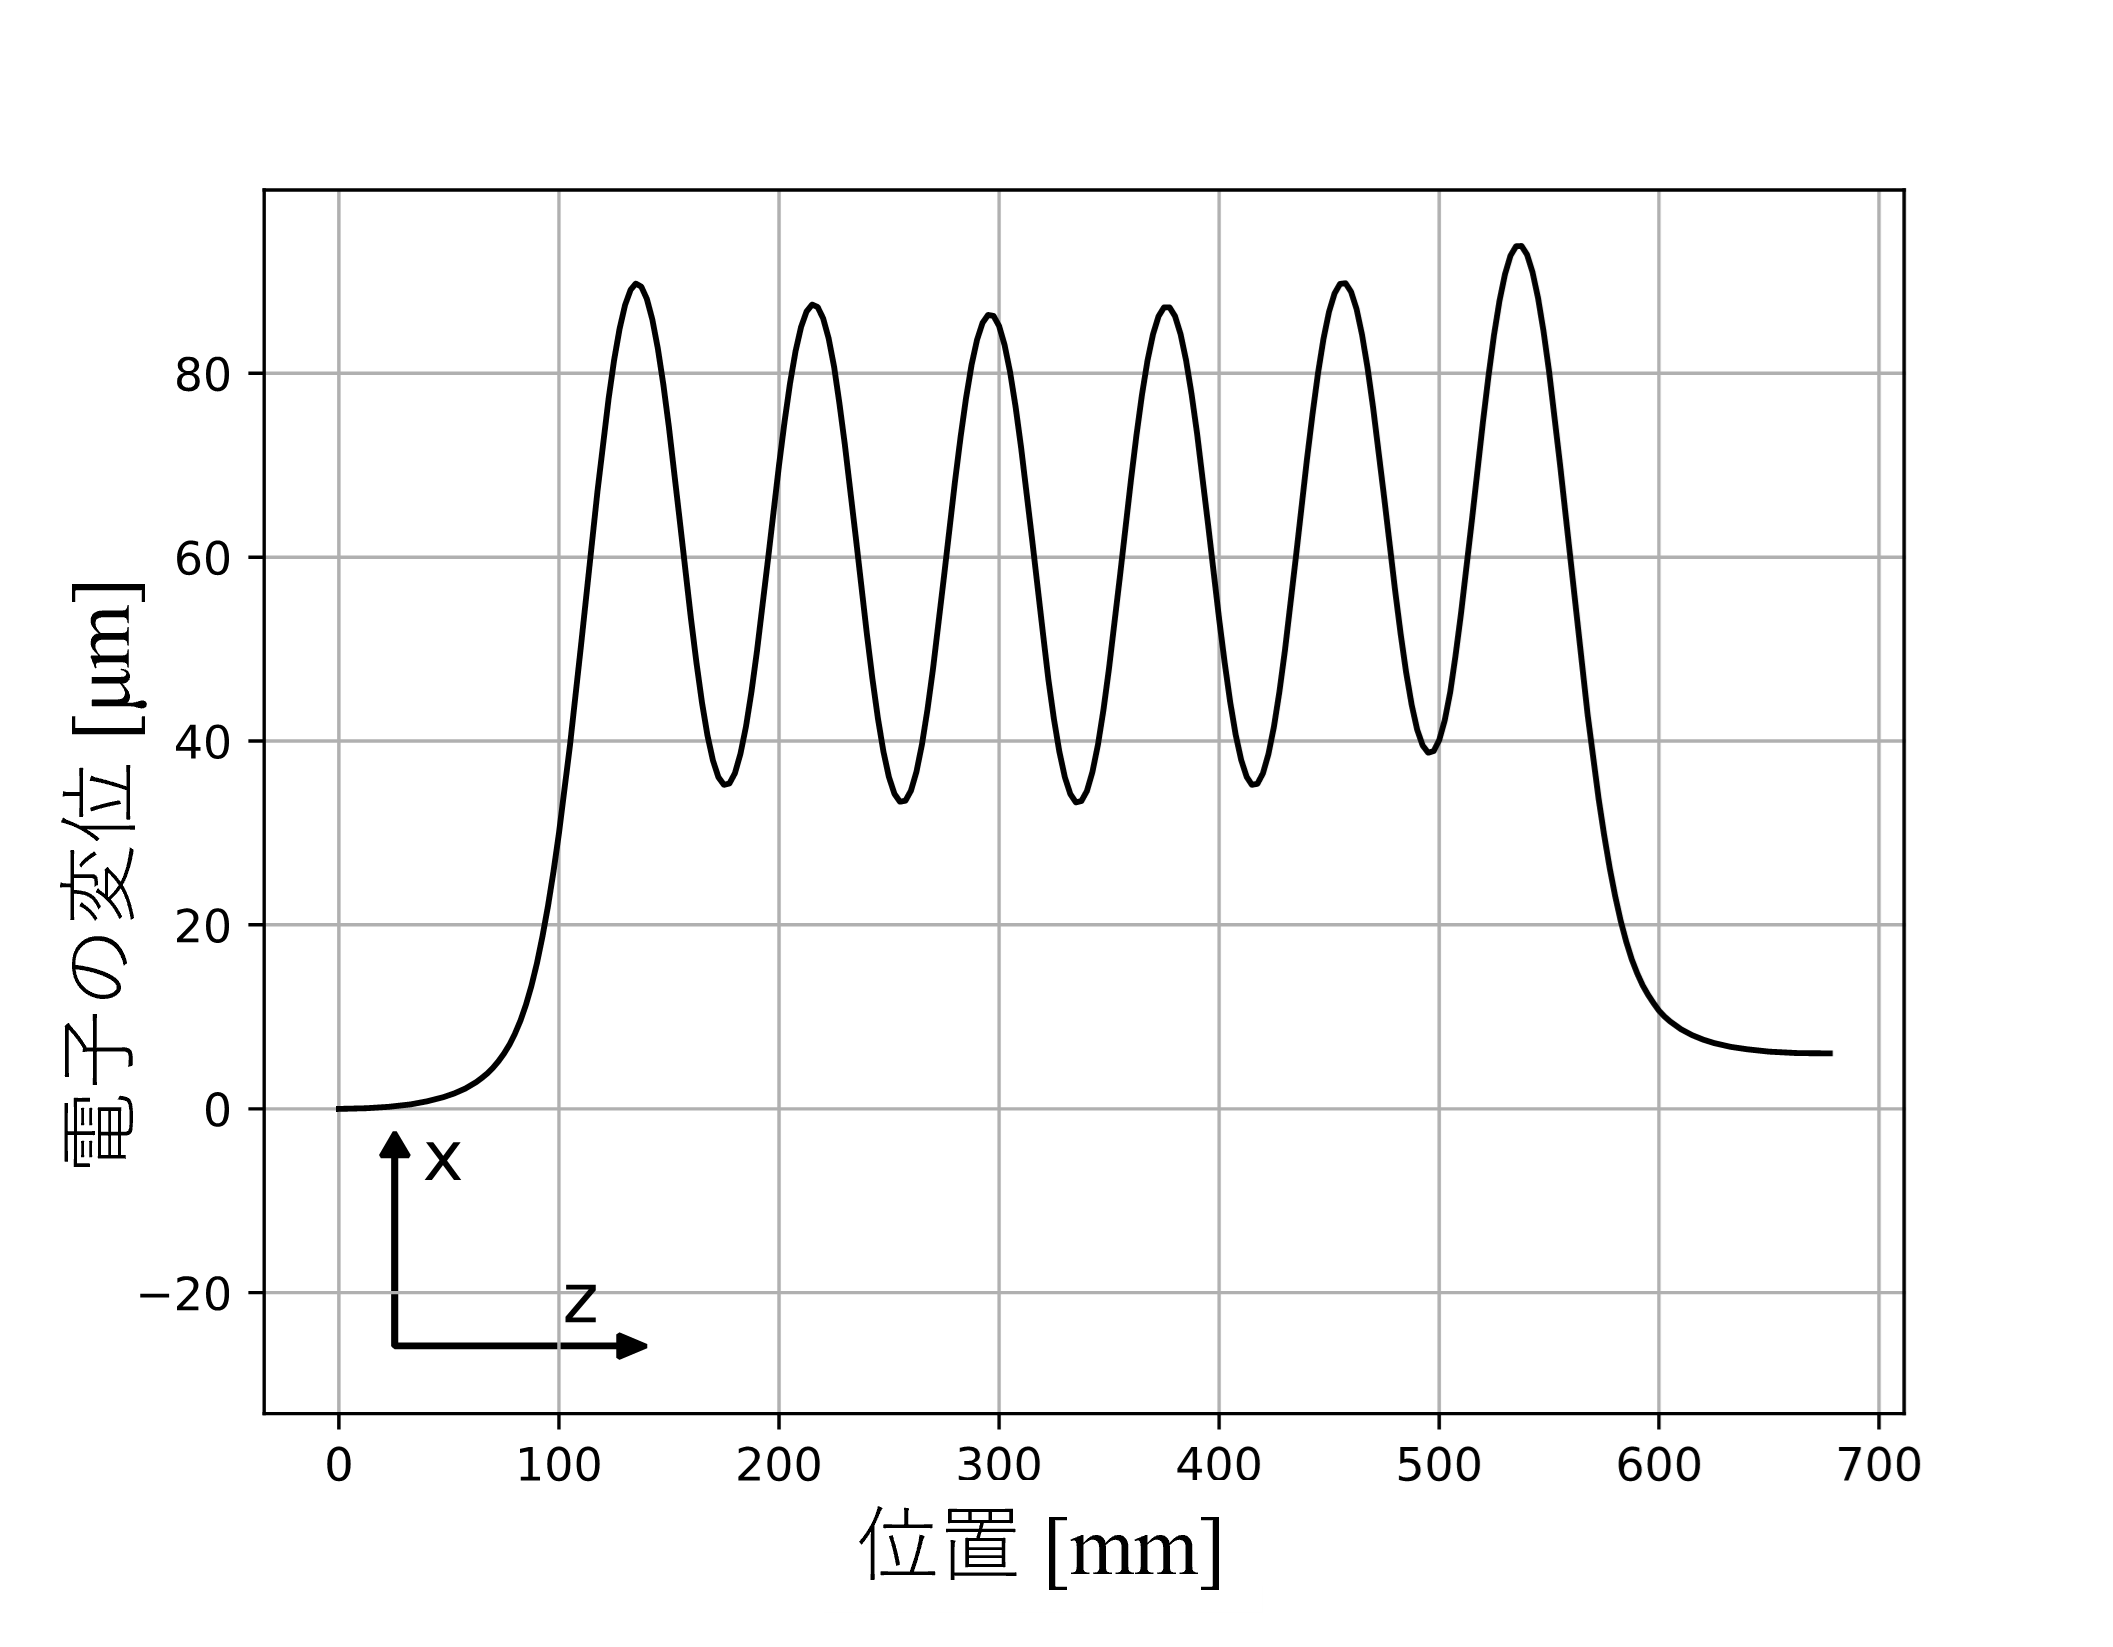
\includegraphics[width=\linewidth]{image/3-undulator_position.png}
    \subcaption{電子軌道の推定値}
  \end{subfigure}
  \caption[ホールプローブによる磁場測定の結果]{E = 180 MeVの時の磁場測定(B = 95~mT)の結果を示す。調整の結果、電子軌道の変位は10~$\mu$m以下に抑えられている。}
  \label{fig:magnetic}
\end{figure}
最後に、電子ビームエネルギーに対する目標磁場と偏向定数、および共鳴波長(放射光の共鳴波長=式(\ref{eq:resonance_wl}))を表\ref{undulator_setting}に示す。
\begin{table}[H]
  \centering
  \begin{tabular}{c|ccc}
    エネルギー [MeV]& 磁場設定値[mT]&偏向定数 $K$&共鳴波長 [nm]\\ \hline
    180 & 95  & 0.710 & 403.6\\
    195 & 130 & 0.971 & 404.2\\
    210 & 140 & 1.046 & 366.4\\
  \end{tabular}
  \caption[アンジュレータの磁場設定値]{アンジュレータの磁場設定値と偏向定数および共鳴波長(放射光のピーク波長)。
  180 MeVおよび195 MeVでは較正波長の404 nmと共鳴波長がほぼ一致したセットアップを実現できたが、210 MeVではアンジュレータのコイルの過電流を避けるために
  共鳴波長を短くする必要があった。}\label{undulator_setting}
\end{table}

\subsubsection{位置制御と読み取り}
アンジュレータは可動式ステージに取り付けられており、モーターによって移動させる。
可動範囲はビームライン上の制約から最大 825~mmに制限されており、間隔は通常の測定では 5 mmで指定する。
移動したアンジュレータの絶対値は、リニアエンコーダ(Heidenhain LC415)で 5 $\mu \text{m}$ の精度で読み出す。

\subsubsection{アラインメント}
セオドライトを用いてアンジュレータと較正用水銀灯、スリットの位置を調整した。セオドライトの基準は四重極電磁石(Q2, Q3)の中心で、この2点を通る直線をビームラインおよび光軸の基準としている。
アンジュレータの設置の際には、基準線をセオドライトを通して見ながら、アンジュレータの上流、下流側の磁石の中心を$x,y$方向に調整可能な調整ステージを動かして調整した。
%四重極電磁石はマーカーを基準に精密に水平に設置されていることが保証されている。
%~~よりも良い精度で水平に設置されている。

\subsection{分光光学系}
分光光学系全体の構成を図\ref{fig:optics}に示す。各素子間の長さは、素子の中心同士を結ぶ直線を測定した。
放射光の光軸が必ずしも素子の中心を通ることは保証されていないことと、放射光はスリットの大きさに対応して数~mm$^2$程度の広がりを持って入射するため、
実効的な距離は実測値と比較して最大10 mm程度のずれが生じると見積もった。
\begin{figure}[h]
  \centering
  \includegraphics[width=\linewidth]{image/3-optics.png}\\
  \caption[分光光学系の全体図]{分光光学系の全体図。光学素子間の長さの単位は mmである。}
  \label{fig:optics}
\end{figure}

\subsubsection{スリット}
矩形スリットを用いる。
スリット幅は4 mm($x$) x 6 mm($y$)であり、調節ねじにより上下、および左右のブレードが連動して動き、スリット幅を調整可能である。
これを$x$軸、$y$軸方向の可動ステージに乗せることでスリット全体の位置を0.1 mm単位で調整可能にした。

\subsubsection{回折格子}
回折格子はThorlab製の回折格子\cite{grating}を用いた。格子定数は1200/mm、大きさは50$\times$50~mm$^2$である。ピッチ・ヨー方向に調節可能な光学マウントによって固定され、さらに光学マウントが水平方向の回転ステージに設置されている。
これにより分光された放射光がカメラ方向に水平に反射されるよう調整できる。

\subsubsection{波長分散レンズ}
水平方向にのみ光波を収束するシリンドリカルレンズを用いた(図\ref{lens})。
大きさは40$\times$50~mm$^2$、焦点距離は1 m である。350 - 410 nmの波長領域に対してARコーティングが施されている。
このレンズもピッチ・ヨー方向および$y$軸方向の調節が可能な光学マウントによって固定される。
\begin{figure}[H]
  \centering
  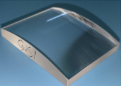
\includegraphics[width=0.4\linewidth]{image/3-lens.png}
  \caption[シリンドリカルレンズ]{シリンドリカルレンズ。水平方向のみに光波を収束し、垂直方向には窓として作用する。}
  \label{lens}
\end{figure}
水平墨出しレーザーの反射光を用いることでピッチ・ヨー回転の調整ができる。

\subsubsection{CMOS カメラ}
光学系は波長が400 nmの領域において動作するため、可視光領域のカメラを用いることができる。HAMAMATSU C14440-20UPを用いた。
仕様を以下に示す。
\begin{table}[h]
\centering
\begin{tabular}{c|c}
  ピクセル数 & 2304 $\times$ 2304\\
  ピクセルサイズ & 6.5 $\mu$m $\times$ 6.5 $\mu$m\\
  チップサイズ & 14.976 mm $\times$ 14.976 mm\\
  ビット深さ & 16 bit\\ 
\end{tabular}
\caption[CMOSカメラの仕様]{CMOSカメラ HAMAMATSU C14440-20UP の仕様}
\end{table}

\subsection{光学系のアラインメント}
青色レーザを用いて光学系全体の光軸調整を行った。青色レーザーの光軸はセオドライトを用いてビームライン中心と合わせる。
ビーム中心と合わせた青色レーザー光を光学系に通し、各光学素子の中心をとおるようにアラインメントを行う。
またレーザー墨出し器を用いて光学系全体の水平を確認する。回折格子とレンズの水平は青色レーザー光の位置を基準に調整した。
青色レーザーはミラーボックスの横20~cmの位置に設置され、次節で説明する水銀灯の較正にもミラーボックスを利用できるようモーターで横方向に移動可能である(図\ref{laser})。
\begin{figure}
  \centering
  \includegraphics[width=0.8\linewidth]{image/3-laser.png}\\
  \caption[青色レーザー]{青色レーザーと水銀灯用スリット。セオドライトを通してミラーボックスを目で見て、ビームライン中心にアラインメントした。}
  \label{laser}
\end{figure}
\section{データ取得}


\subsection{分光光学系の波長較正}
波長較正として水銀灯を用いる。
$400 \text{nm}$領域には2本の輝線があり、このスペクトルを光学系で観測することで2つの輝線スペクトルを観測できる。
水銀灯ランプはビームラインから垂直に5 mの位置に設置されており、ミラーボックス内のミラーを用いて電子ビームラインと同じ軌道を通って光学系に導かれる(図\ref{mirrorbox})。
ミラーボックスの直前には水銀灯用の円形スリットを設置した(図\ref{laser})。

輝線スペクトルをガウス関数でフィッティングし、中心位置のピクセルを対応する波長にする。
2本のスペクトル以外のピクセルは2本の輝線の波長 -ピクセル関係の線形性を仮定して決定する。
\subsection{データ取得}\label{sec:DAQ}
以下の手順を繰り返してデータ取得を行う。
ステージモータに指定する位置の値は0から825~mmの範囲で、5~mm間隔、計166点である。
\begin{itemize}
  \item アンジュレータのステージモータに次の指定位置の信号が送られる
  \item 指定の位置にアンジュレータが移動する
  \item カメラによる画像撮影の信号が4回送られる
  \item 画像撮影が完了し4枚の画像が追加されたことをDAQが確認する
\end{itemize}
同時にリニアエンコーダの位置読み出しも行い、データがラズベリーパイに保存される。この流れを図\ref{DAQ}に示す。
\begin{figure}
  \centering
  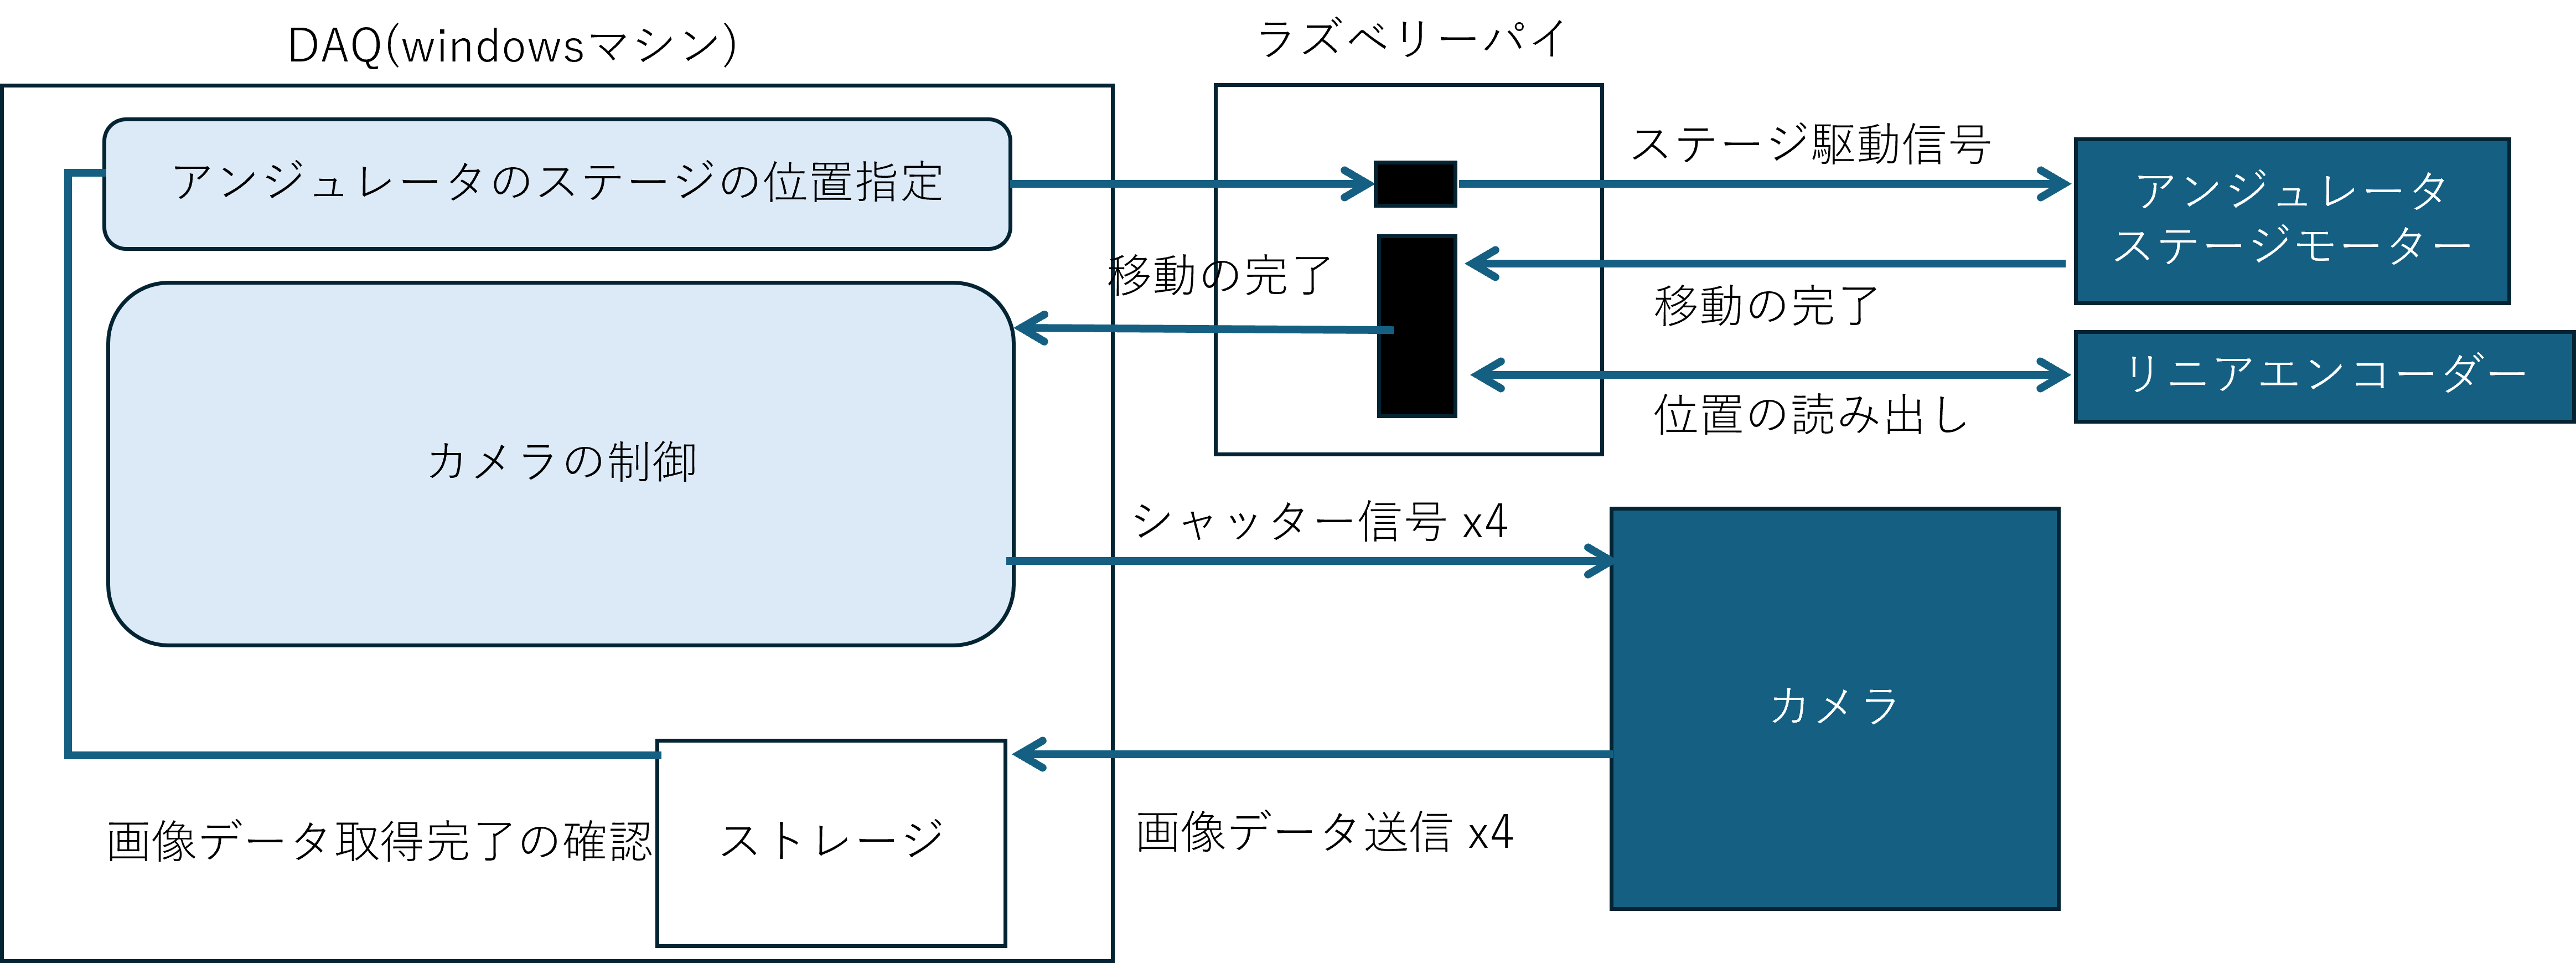
\includegraphics[width=0.8\linewidth]{image/3-DAQ.png}\\
  \caption[データ取得の流れ]{データ取得の流れ。アンジュレータが指定位置に移動するとカメラによる画像撮影が行われる。画像撮影が完了するとDAQに信号が送られ、次の指定位置にアンジュレータが移動する。
  ステージの移動が完了したらラズベリーパイからリニアエンコーダーに位置読み出しの信号が送信され、位置データがラズベリーパイへと送信される。これを166回繰り返すと1つのデータセットが取得できる。}
  \label{DAQ}
\end{figure}
\subsection{弾性散乱実験との同時運用における電子ビームエネルギー測定}

今回の実験の目的は弾性散乱実験における電子ビームエネルギーの精密測定である。この目的に照らし合わせて、弾性散乱実験でのデータ取得の前後にエネルギー測定を行うランプランを設定した(図\ref{beamtime})。
\begin{figure}
  \centering
  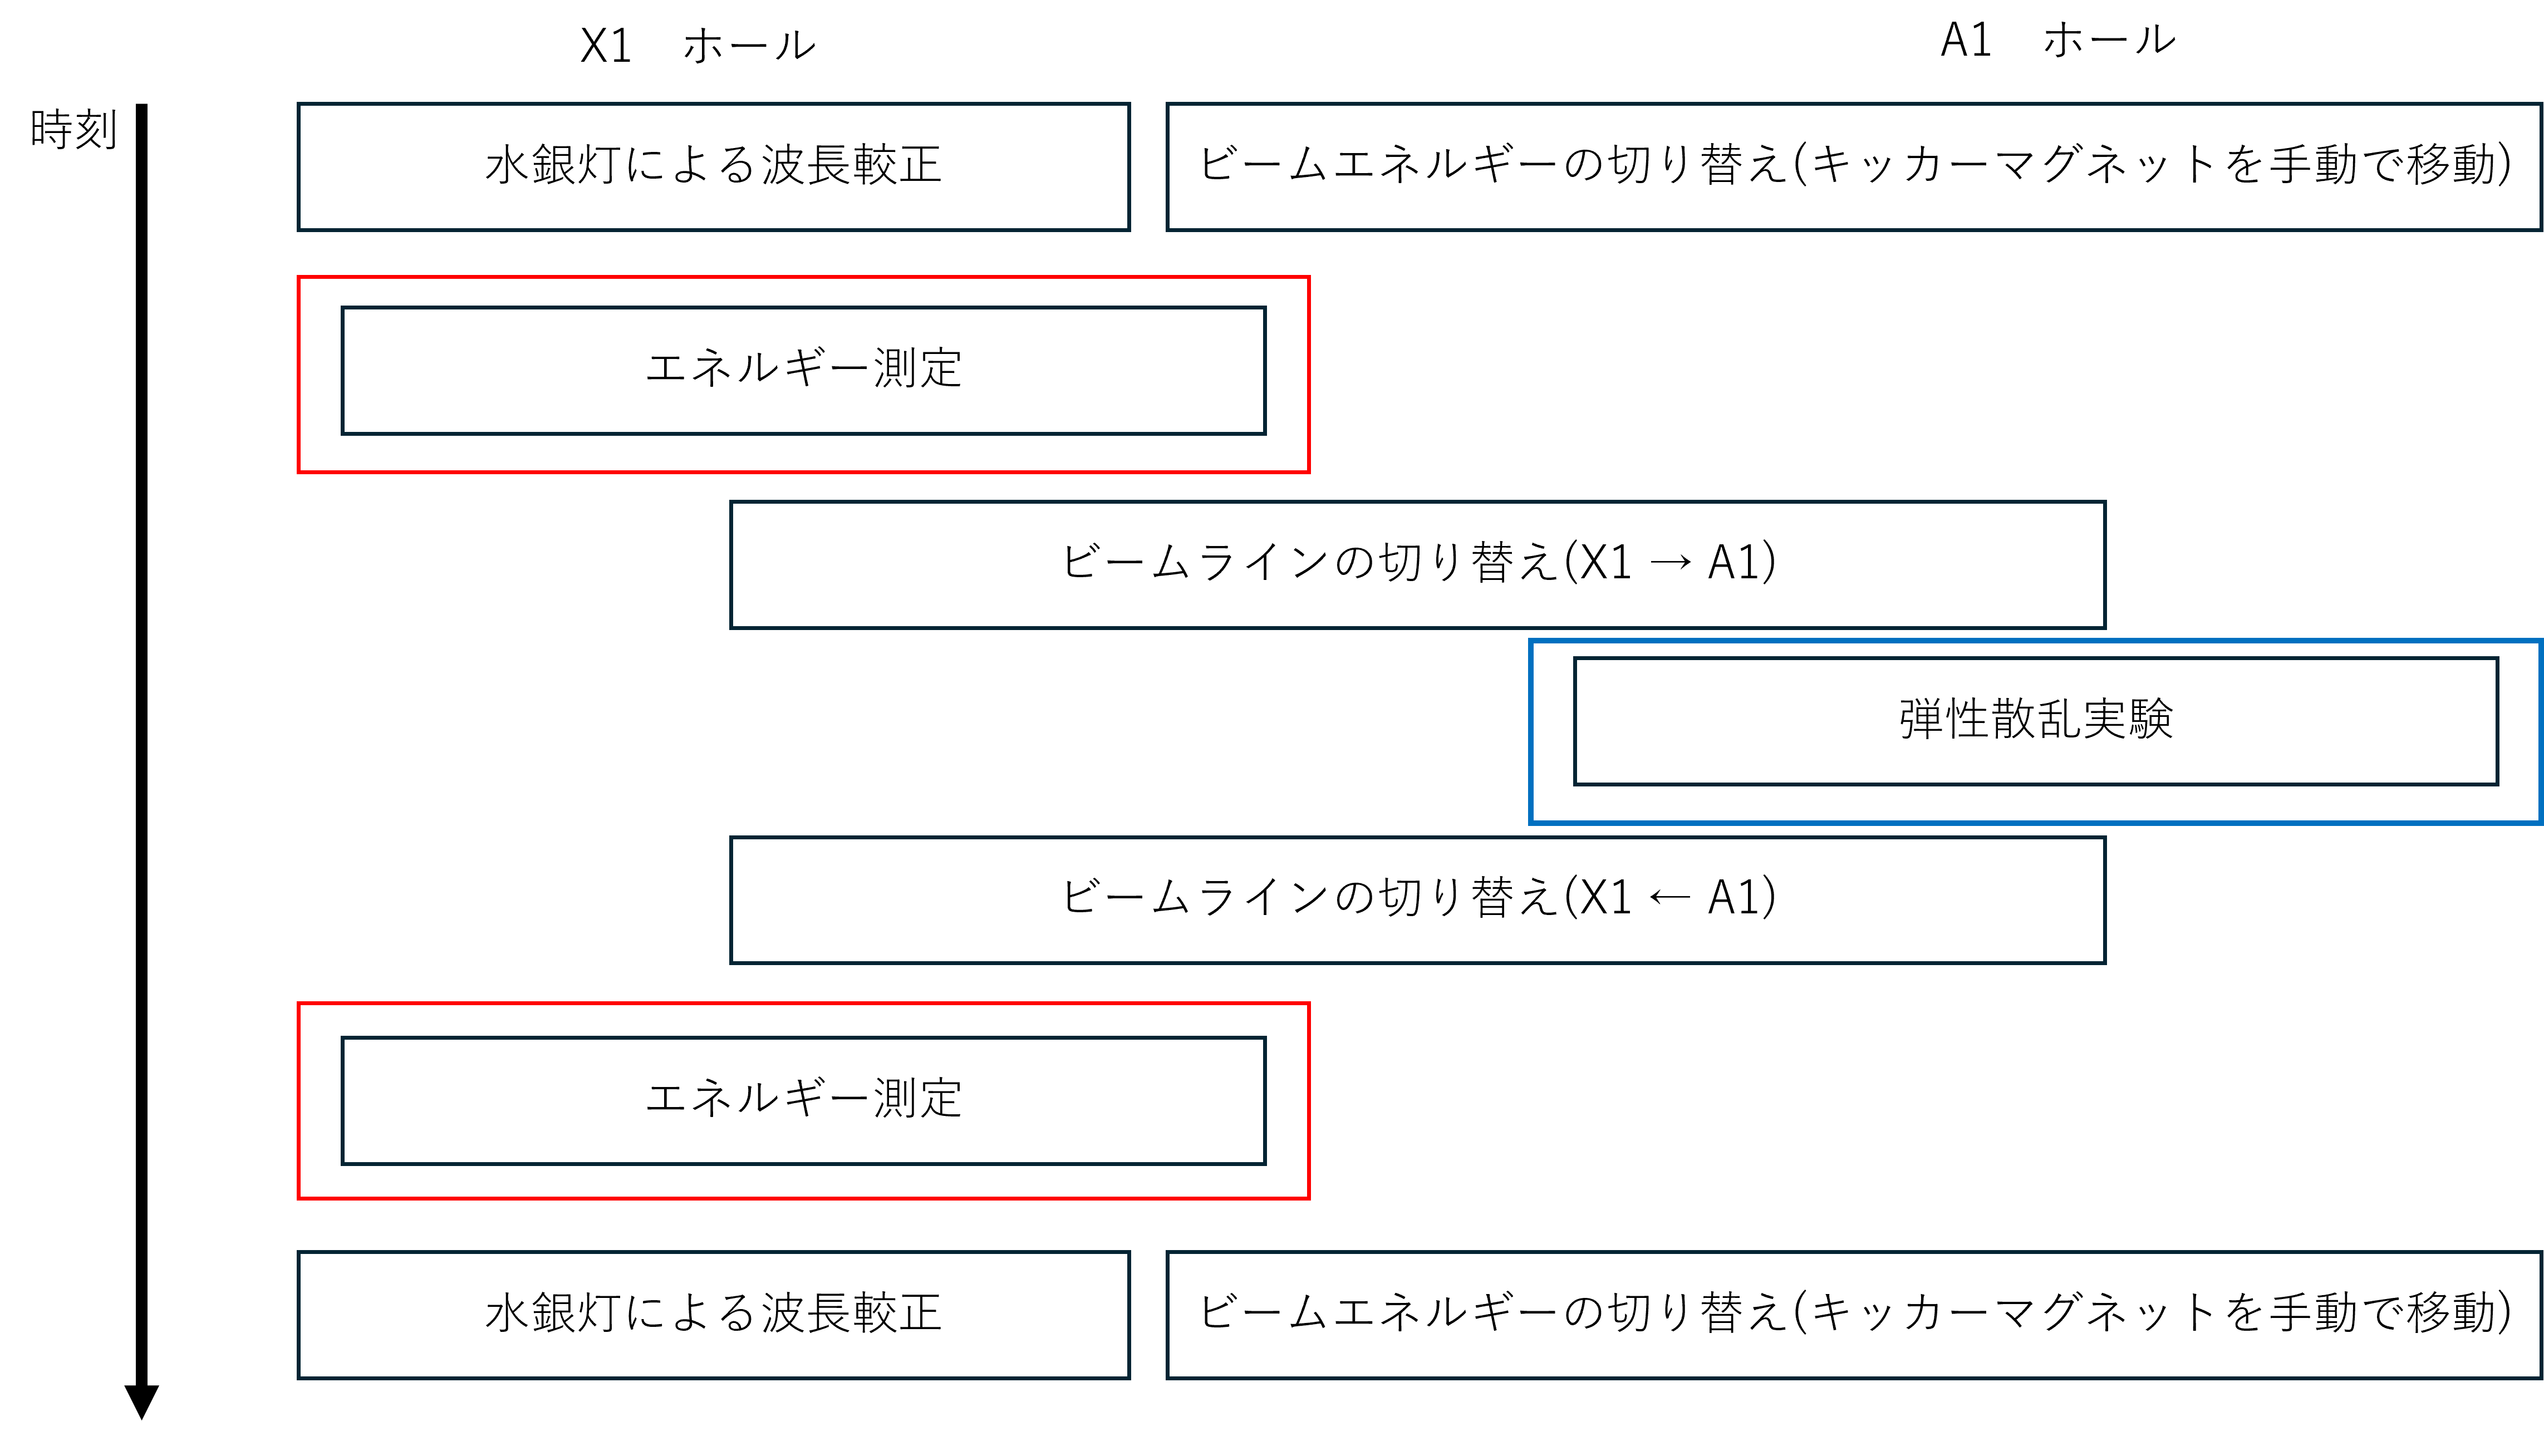
\includegraphics[width=\linewidth]{image/3-beamtime.png}\\
  \caption[弾性散乱実験とエネルギー測定の同時運用]{弾性散乱実験とエネルギー測定の同時運用。弾性散乱実験の前後にエネルギー測定を行う。赤、または青で枠の色がつけられている時間帯がビームが照射されている時間である。
  黒の枠で囲われた時間帯は、実験ホールでの作業と、一部ビーム調整の時間が含まれており、データ取得はできない。また「エネルギー測定」の内容は前節\ref{sec:DAQ}で述べたとおりである。}
  \label{beamtime}
\end{figure}
\subsection{下流側アンジュレータによるデータ測定}
パラメータ較正を目的として、下流側アンジュレータのみを用いたデータ取得を行う。
実験条件は$E_{beam} = 210$~MeVで、アンジュレータの磁場は140~mTとした。

上流のアンジュレータ(赤)はコイルに流す電流を0にしたうえで、残留磁場の影響を受けないように$x$軸方向に30~cmずらした。

\end{document}
\documentclass[a4paper,11pt,uplatex]{jsarticle}


% 数式
\usepackage{amsmath,amsfonts}
\usepackage{bm}
\usepackage{physics}
% 画像
\usepackage[dvipdfmx]{graphicx}
\usepackage[dvipdfmx,colorlinks=true,linkcolor=blue]{hyperref}
\usepackage{pxjahyper}

\begin{document}


\section{モデル関数によるフィッティング}
\subsection{放射光}
アンジュレータ放射光の振幅は放射角の関数として以下のように計算できることが知られている。
また放射光の位相は球面波を仮定する。

\subsection{フレネル回折}
放射光がスリットを通過すると回折を受け、特徴的な縞模様が現れる。回折現象は以下のレイリーゾンマーフェルト積分によって厳密に計算することができる
\begin{eqnarray}
  \text{U}(\text{P}) = \frac{1}{4\pi}\int_{S}\cos(ns)\text{U}(S)\frac{\exp(iks)}{s}\left( ik - \frac{1}{s}\right) -U(S)\frac{\exp(iks)}{s}\left(ik- \frac{1}{r}\right)\cos(nr) dS
\label{レイリーゾンマーフェルト}
\end{eqnarray}
近似① $k \gg 1/r$, $k \gg 1/s$
近似② $\cos(nr) \sim 1$,$\cos(ns) \sim 1$
近似③ 領域Sにおいて$r(S)= z = \text{const.}$,$s(S) = s_0 = \text{const.}$
により式(\ref{レイリーゾンマーフェルト})は
\begin{eqnarray}
  \text{U}(P) = -\frac{i}{2\lambda rs} \int_{S} U(S)\exp ik(r+s) dS
  \label{レイリーゾンマーフェルト近似}
\end{eqnarray}
\begin{eqnarray}
  \text{U}(P) = -\frac{i}{2\lambda rs} \int_{S} U(S)\exp ikr dS
\end{eqnarray}
このような回折現象は伝搬距離によっては近似計算できることが知られている。以下では積分領域$S$上の座標を$x,y$、観測点Pの座標を$x_0,y_0$と表記する。
\begin{eqnarray}
  r &=& \sqrt{z^2 + (x-x_0)^2 + (y-y_0)^2}\\
  &=& z + \frac{1}{2}\frac{(x-x_0)^2 + (y-y_0)^2}{z} - \frac{1}{8}\frac{\left[(x-x_0)^2 + (y-y_0)^2\right]^2}{z^3} +\dots
\end{eqnarray}
$\left[(x-x_0)^2 + (y-y_0)^2\right]^2 \ll z^3$が成立するなら
\begin{eqnarray}
  \text{U}(x_0,y_0) \sim -\frac{i}{2\lambda zs_0}\int \text(U)(x,y) \exp(ik\left\{z +\frac{1}{2}\frac{(x-x_0)^2 + (y-y_0)^2}{z}\right\})
\end{eqnarray}

\subsubsection{数値計算上の計算手法}
数値計算を実行する上では数値積分の手法では、伝搬後のN次元の配列が伝搬前のN次元配列全ての積分を用いて計算されるため計算量は$\text{N}^2$となる。
このような計算コストの高い計算を避けるために、高速フーリエ変換を用いた計算が一般に用いられている。
式(\ref{レイリーゾンマーフェルト近似})を再度$x,y,x_0,y_0$で書き直すと
\begin{eqnarray}
  \text{U}(x_0,y_0) \sim \frac{1}{2i\lambda zs}\int_S \text{U}(x,y) \exp( ik \sqrt{z^2 + (x-x_0)^2 + (y-y_0)^2}) dxdy
\end{eqnarray}
これはカーネル関数$f(x,y) = \sqrt{z^2 +x^2 + y^2}$であるような畳み込みの形で書ける
\begin{eqnarray}
  U(x_0,y_0) \sim (\text{U} * f)(x,y)
\end{eqnarray}
畳み込みはフーリエ変換を用いることで
\begin{eqnarray}
  (U*f)(x,y) = \mathcal{F}^{-1}(\mathcal{F}(U) \times \mathcal{F}(f))
\end{eqnarray}
と表せる。
\begin{eqnarray}
  \mathcal{F}^{-1}(\mathcal{F}(U) \times \mathcal{F}(f)) &= \mathcal{F}^{-1} \left( \int f(x)e^{iwx}dx \times \int g(x)e^{iwx}dx \right) \\
  &= \mathcal{F}^{-1}\left( \right)
\end{eqnarray}

\subsection{電子ビームサイズ}

\subsection{光学系}
回折格子によって分光された光はレンズによってカメラで収束する

\subsection{パラメータ}
求める関数系は放射光関数と光学系関数からなる。
パラメータの定義を以下に示す。
\begin{itemize}
\item$\gamma$ 電子ビームエネルギーのローレンツ因子
\item$\text{K}$ アンジュレータのK値
\item$\text{z(U2-S)}$下流アンジュレータ-スリット間の距離
\item$\text{z(S-C)}$スリット-カメラ間の距離
\item$\text{w(S)}$スリットの鉛直方向の長さ
\item$\text{y(beam)}$カメラに対するビーム中心のy座標
\item$\text{y(slit)}$カメラに対するスリット中心のy座標
\end{itemize}


\subsection{パラメータ較正}
アンジュレータひとつのデータの解析について
アンジュレータ


\subsection{画像処理}
同一条件で4枚の画像を撮影し各ピクセルごとに平均値を取る
ノイジーなピクセルはマスクしてフィッティングの対象に含まない。









\clearpage

\begin{figure}[tb]
  \centering
  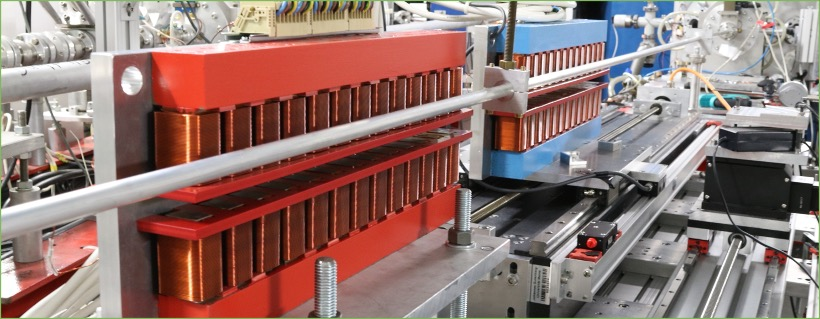
\includegraphics[width=0.8\linewidth]{image/1-1.jpg}\\
  \caption{サンプルの図}
  \label{sample_image}
\end{figure}

\begin{itemize}
  \item a
\end{itemize}
\begin{enumerate}
  \item b
\end{enumerate}

\begin{align}
\frac{1}{2} = \qty(\frac{1}{3}) + \qty{1}\Sigma
\end{align}
\end{document}
%\documentclass[a4paper,11pt,uplatex]{jsarticle}


% 数式
\usepackage{amsmath,amsfonts}
\usepackage{bm}
\usepackage{physics}
% 画像
\usepackage[dvipdfmx]{graphicx}
\usepackage[dvipdfmx,colorlinks=true,linkcolor=blue]{hyperref}
\usepackage{pxjahyper}

\begin{document}


\section{結果}
\subsection{画像処理}
各ピクセルが持つ不定性の結果を示す。

\subsection{単アンジュレータ}
下流側のアンジュレータのみを用いて取得したデータの解析結果を示す。
このデータを用いてパラメータの較正をおこなった。

\subsubsection{放射光および光学系パラメータ}
回折パターンの形状を決定するパラメータはアンジュレータ - スリット間距離、スリット - カメラ間距離、スリット幅の3つである。
これに加えて放射光関数の情報も形状を決定する。

\subsubsection{距離依存性}
アンジュレータと光学系の距離に依存して光量が変化する。
立体角を考えるとこの光量は距離rに対して$\frac{1}{r^2}$に比例する

\subsection{振動パターン}
2つのアンジュレータの放射光による干渉パターンの振動を解析する。


\subsection{系統誤差}
\subsubsection{波長依存性}
異なる波長でエネルギーを決定する

\subsubsection{距離依存性}
下流側アンジュレータの位置を4つの区間に分割し、各区間でエネルギーを決定した。
これによりフィット関数が持つ位置依存性による系統誤差を見積もることができる。

\subsubsection{エネルギー依存性}
180.195,210 MeVの3つのエネルギーの結果












\clearpage

\begin{figure}[tb]
  \centering
  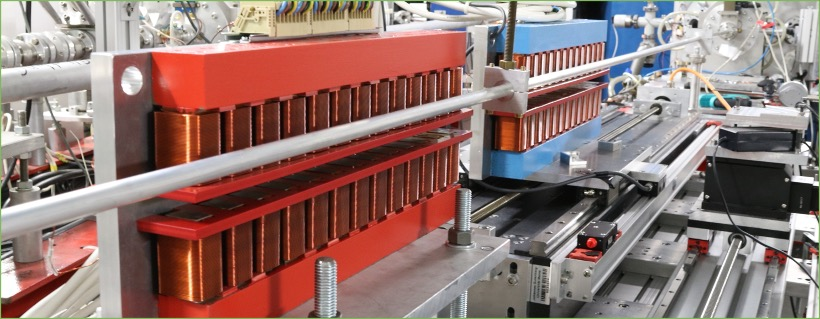
\includegraphics[width=0.8\linewidth]{image/1-1.jpg}\\
  \caption{サンプルの図}
  \label{sample_image}
\end{figure}

\begin{itemize}
  \item a
\end{itemize}
\begin{enumerate}
  \item b
\end{enumerate}

\begin{align}
\frac{1}{2} = \qty(\frac{1}{3}) + \qty{1}\Sigma
\end{align}
\end{document}
\documentclass[a4paper,11pt,uplatex]{jsbook}
%\usepackage{fancyhdr}
\setlength{\footskip}{16pt}
\usepackage{amsmath}
\usepackage[dvipdfmx]{graphicx}
\usepackage[dvipdfmx]{color}
%\usepackage{pagecolor}[white]
\usepackage{amsmath,amssymb}
%\usepackage[top=3cm, bottom=3cm, left=3cm, right=3cm]{geometry}
\usepackage{braket}
\usepackage{bm}
\numberwithin{equation}{section}
\usepackage{mathrsfs}
\usepackage{siunitx}
\usepackage{physics}
\usepackage[dvipdfmx]{graphicx}
\usepackage[compat=1.1.0]{tikz-feynhand}
\usepackage{caption}
\usepackage{subcaption}
%\usepackage{cleveref}
\usepackage{float}
\usepackage{multicol}
\setlength{\columnsep}{15mm}
%\usepackage[style=phys,articletitle=false,biblabel=brackets,chaptertitle=false,pageranges=false]{biblatex}
%\usepackage[style=phys]{biblatex}
\usepackage[dvipdfmx]{hyperref}
\usepackage{url}
\usepackage{pxjahyper}
\usepackage{bookmark}
%\usepackage[backref]{hyperref}
\setcounter{tocdepth}{3}
\setlength{\parindent}{2em}
\def\vector#1{\mbox{\boldmath $#1$}}
\def\slash#1{\not\!#1}
\def\slashb#1{\not\!\!#1}
\def\delsla{\not\!\partial}
%\usepackage[dvipdfmx]{xcolor}


\hypersetup{
 setpagesize=false,
 bookmarksnumbered=true,%
 bookmarksopen=true,%
 colorlinks=true,%
 linkcolor=black,
 citecolor=red,
 urlcolor=black,
}
%backreferenceのカスタマイズ. "Back to p.3"のように表示する.
%\renewcommand*{\backref}[1]{(p.#1へ戻る)}
%\newcommand{\backtoc}{\hyperlink{toc}{[目次へ]}}
\newcommand{\backtoc}{\texorpdfstring{\protect\hyperlink{toc}{\hspace{5pt} \scriptsize [目次へ]}}{}}
\newcommand{\mychapter}[1]{\chapter[#1]{#1\backtoc}}
\newcommand{\mysection}[1]{\section[#1]{#1\backtoc}}
\newcommand{\mysubsection}[1]{\subsection[#1]{#1\backtoc}}

% 数式
%\usepackage{amsmath,amsfonts}
%\usepackage{bm}
%\usepackage{physics}
% 画像
%\usepackage[dvipdfmx]{graphicx}
%\usepackage[dvipdfmx,colorlinks=true,linkcolor=blue]{hyperref}
%\usepackage{pxjahyper}

\begin{document}

\chapter{考察}
\section{考察}
\subsection{光学系}
回折パターンを決定する要素として放射光関数と光学系関数がある。
エネルギーを求めるには放射光の情報が分かれば良いが、今回は放射光関数を仮定している。
光学系関数の光学計算は原理的には正確に計算可能である
光学系によって、分光された光の情報から入射光の情報を逆演算する系を構築することができれば精度の向上につながる

\subsection{汎用的な電子ビームエネルギー測定手法としての改善点}

\subsection{原子核実験との同時測定}





\clearpage

\begin{figure}[tb]
  \centering
  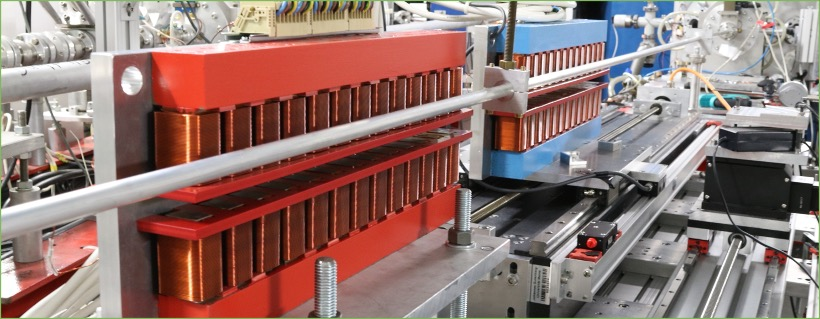
\includegraphics[width=0.8\linewidth]{image/1-1.jpg}\\
  \caption{サンプルの図}
  \label{sample_image}
\end{figure}

\begin{itemize}
  \item a
\end{itemize}
\begin{enumerate}
  \item b
\end{enumerate}

\begin{align}
\frac{1}{2} = \qty(\frac{1}{3}) + \qty{1}\Sigma
\end{align}
\end{document}
%\appendix
\printbibliography[title=参考文献]
%\bibliography{ref}
%\bibliographystyle{unsrt}
\end{document}